
\chapter{EcoDrive: A Mobile Sensing and Control System for Fuel Efficient Driving}
\label{chapter_ecodrive}

In this chapter, we introduces EcoDrive, 
a fuel consumption sensing and control system for modern vehicles, implemented
in an embedded platform, to improve fuel efficiency and reduce carbon emissions. 
EcoDrive senses vehicle dynamics
through the standard vehicle On-board diagnostics (OBD)
port and models various vehicle forces, i.e., propulsion, drivetrain loss, 
wind resistance and grade resistance, as functions of instant fuel consumption. 
By sensing vehicular speed and
controlling air/fuel injection rate in real time, EcoDrive can
adjust speed carefully to improve fuel efficiency.
We start with a background of vehicle system, followed by modeling
of vehicle dynamics and fuel consumption rate, and
then we will present a dynamic programming algorithm
to find tradeoffs between travel time and fuel efficiency. 

\section{Preliminaries}





To illustrate how vehicle system works 
and how each components are related to different OBD parameters,
we present a high-level vehicle system control 
flow in Fig. \ref{vehicle_system}. 
Drivers accelerate vehicle by pressing the gas pedal, 
and then the gas pedal position will be sent to 
the Electronic Control Unit (ECU). 
The ECU controls air/fuel injection rate
to produce engine torque to drive the vehicle.   
Transmission is used in this process 
to transit power from engine to wheel and 
match engine rotational speed with wheel rotational speed. 


\begin{figure}[t]
\begin{center}
\vspace{-0.0cm}
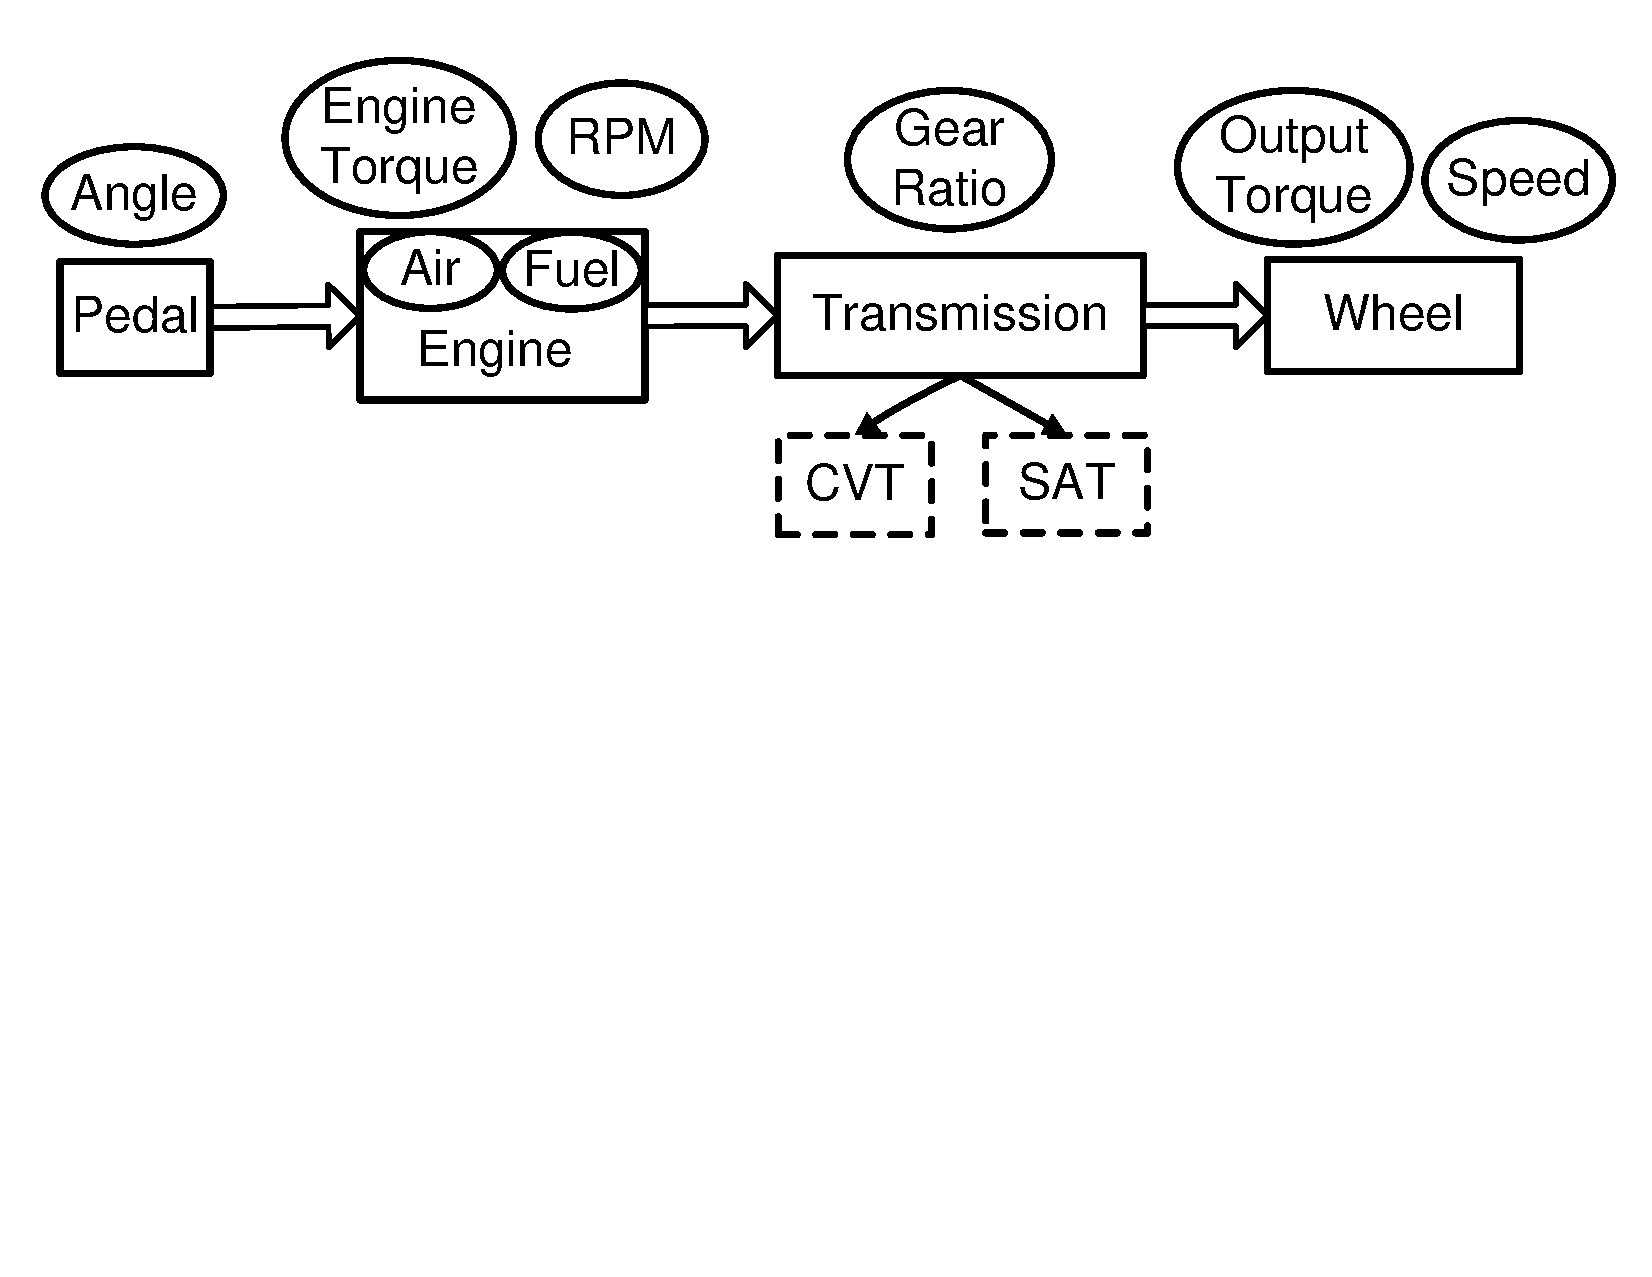
\includegraphics[width=5.0in,angle=0]{Figs/EcoDrive/drivetrain.pdf}
\vspace{-5.5cm}
\caption{Vehicle Drivetrain.}
\vspace{-0.5cm}
\label{vehicle_system}
\end{center}
\end{figure}


\subsection{Power Production and Transition}

In a car engine, the explosion of compressed fuel and air 
produces the power to drive a car.
The air is injected through an intake port and expelled from an exhaust port.
The volume of oxygen in the exhaust air is monitored by fuel trim sensors. 
Based on fuel trim sensor readings, the Electronic Control Unit (ECU) 
calculate the desired fuel injection rate to maintain the
ideal air/fuel ratio 
\footnote{Air/fuel ratio is a constant value around 14.67, 
while air/fuel rate is the volume of air/fuel injected per unit time.}. 


The burning of air and fuel mixture triggers the revolution of 
crankshaft, which carries piston power out of the engine to the transmission.
The transmission carries power to wheels.  
Transmission is also known as gearbox that uses gears and gear trains
to provide speed and torque conversion. 
The transmission reduces the higher engine speed to the slower
wheel speed and increases torque in the process of accelerating the vehicle. 
The transmission converts engine revolutions to driveshaft revolutions, and then to axle revolutions.
A Continuously Variable Transmission (CVT) is a 
transmission that can change 
seamlessly through an infinite number of effective gear ratios 
between maximum and minimum values. 
This contrasts with Step 
Automatic Transmissions (SAT) that offer a fixed number of gear ratios.

\subsection{OBD Parameters}

On-board diagnostics (OBD) is an automotive 
term referring to a vehicle's 
self-diagnostic and reporting capability.  
It is the interface between car Controller Area Network (or CAN bus) and external devices, 
e.g., a OBD scan tool that connects the OBD port and a laptop. 
Car CAN bus allows vehicular components to communicate with each other. 
For example, a position value is sent to 
the Electronic Control Unit (ECU) after human driver
press the gas pedal, 
and the ECU adjusts air/fuel injections according to the position value.
Therefore, we can read this position message transmitted over CAN bus 
from the OBD port. 





The data we collected from the OBD port are summarized in Table \ref{obd_data}. 
Fuel Level (FL) of the vehicle is usually measured by a float sensor, 
which is usually visualized on the fuel gauge in the car \cite{fuel-gauge}.
The FL is calculated according to the height of the float. 
\nop{
When fuel is injected into the tank, the fuel will raise 
the float up, and vice versa. 
This mechanism makes the FL measurement is not accurate
and can be only used to long-term fuel consumption estimation. 
For example, the float may reach the top of the tank even 
before the tank is filled up.
The fuel gauge will show a full tank even 
when more fuel is possible to be filled.  
Similar thing happens when the fuel tank close to empty. 
}
The Fuel System Status (FSS) is used to indicate current engine mode, 
open loop mode or closed loop mode. 
In open loop mode, 
the engine calculate the fuel injection based on the pre-calculated
table and there is no feedback to the engine to adjust the fuel injection rate. 
The engine runs in open loop mode during short warm up time
and runs in closed loop mode at most of the time. 
In closed loop mode, the engine adjusts fuel injection rate based on
fuel trims and air flow rate. 
Mass Air Flow Rate (MAF) is used to measure the air intake rate of the engine, 
and therefore an effective indicator of instant fuel consumption 
\cite{alessandrini2012consumption, lee2011estimation, koukoumidis2011signalguru}. 
Both Long Term Fuel Trim (LTFT) and Short Term Fuel Trim (STFT) are used to 
adjust the air/fuel rate injected into engine. 
LTFT changes less frequent than STFT. 
We use AFR as a metric of 
instant fuel consumption and/or carbon emission. 


\begin{equation}
AFR = C_f * MAF * (1 + LTFT) * (1 + STFT).
\end{equation}

where $C_f$ is a constant value for unit conversion, e.g., from air flow rate to
fuel rate or to carbon emission rate. 

Vehicular Speed is measured by the perimeter of the wheel and 
number of rotations. 
Accelerator Position is measured by the angle of the gas pedal.
It controls the air/fuel rate injected into the Engine.  
Engine RPM is measured by the rotation speed of the engine motor. 


\subsection{Dataset}



\begin{figure}[t]
\begin{center}
%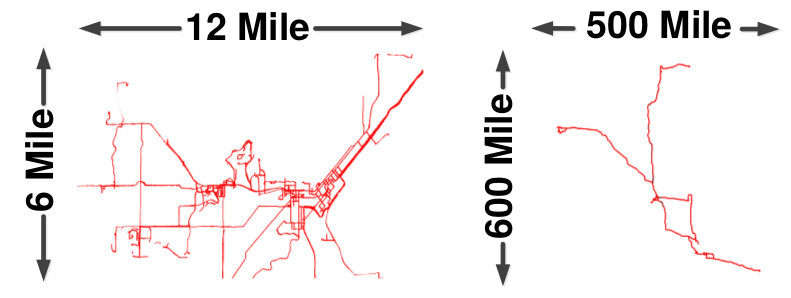
\includegraphics[width=3.0in, angle=0]{Figs/EcoDrive/urbanhighwaymap.png}
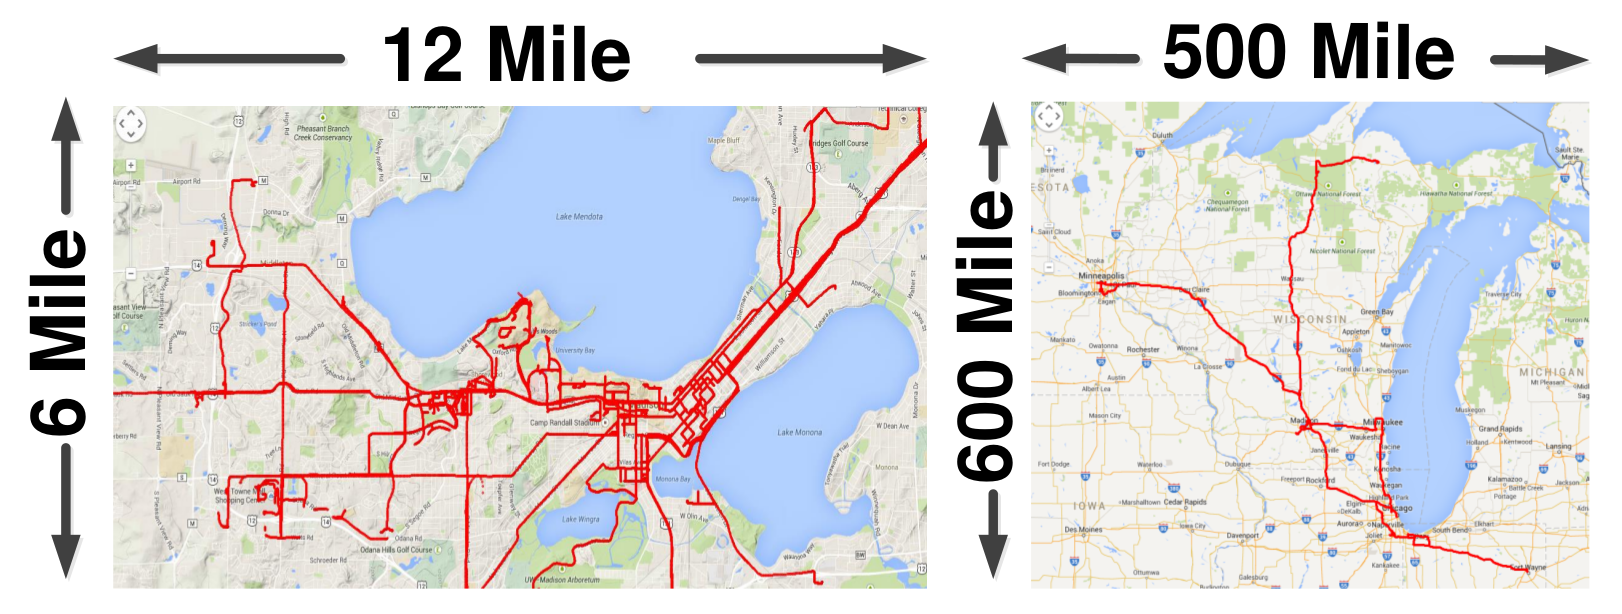
\includegraphics[width=5.0in, angle=0]{Figs/EcoDrive/map.png}
\vspace{-0.0cm}
\caption{Urban driving data (left) is collected from a US mid-size city.  
Highway driving data (right) is collected from both local highways and cross-state highways.}
\vspace{-0.5cm}
\label{rpm_gph}
\end{center}
\end{figure}


%The map area is about 600 mile $\times$ 500 mile.
%The map area is about 6 mile $\times$ 12 mile. 


We use a customized Android application to collect OBD and GPS data 
from different car makes and models.
The dataset is summarized in table \ref{vehicles}.
The transmission of car 2,6,9,10 and 11 is CVT and the rest is SAT. 
The driving data of car 1-6 is collected over a course of three months, 
and the rest is collected from random events, 
e.g., three cross-state highway trips are collected by car 7, 8 and 9, 
respectively. 
Here we separate urban driving and highway driving,
as urban driving patterns are dominated by frequent 
accelerations and decelerations while 
highway driving patterns are dominated by 
constant speed cruising. 
The dataset covers car makes from three different countries, 
urban data over 5,000 miles, highway data across 5 US states and 
over 5,000 miles, two common types of transmissions. 
We use the first car to install a prototype of EcoDrive and tested
it in both urban and highway environments. 
%EcoDrive is tested on Madison's West Betline Highway, between exit 257 and 261. And US 14 Highway between exit 132 and 136.




\subsection{EcoDrive Architecture}

EcoDrive reads real-time OBD parameters through OBD port
and controls air/fuel injection rate by emulating the gas pedal.
We illustrate the architecture of EcoDrive in Fig. \ref{ecodrive}.
The sensed parameters from OBD port are passed to modeling component
to train the models.
The modeling component builds an AFR profile to 
record the instant fuel consumptions of various 
accelerations at different speeds.
Based on pre-calculated driving strategy and real-time sensed vehicular speed, 
the controlling component controls air/fuel injection rate to adjust vehicular speed by 
sending the gas pedal position values to the ECU. 
To emulate the gas pedal, we utilize the drive-by-wire technology, 
where the gas pedal and throttle are connected by electronic messaging instead of mechanical linkage.   
It enables the position of gas pedal can be sent as a message
to control throttle position. 
The throttle controls the volume of air flow injected into the engine. 
 


\subsection{Applications}

EcoDrive is used as an independent system that can be installed
on regular vehicles.  
It can be used as a control system in a way similar to 
cruise control \cite{cruise_control, bengtsson2001adaptive, ioannou1993autonomous}. 
In this application, it is used as a EcoDrive mode that a human driver
can switch it on or off. 
Drivers are required to press the brake pedal to turn this mode off
to keep safe distance to front car or traffic lights/signs accordingly.
This mode can be integrated with intelligent front object or traffic light detection
systems \cite{bengtsson2001adaptive, ioannou1993autonomous} 
to further enhance driving experience. 
EcoDrive requires two inputs, the speed limit and road length. 
The speed limit can be specified by human driver or obtained from online database \cite{speedlimit}. 
The road length can be calculated by a navigation software.



It can also be used as a subsystem of autonomous driving systems 
\cite{googledriverlesscar, urmson2008autonomous, litman2013autonomous, kim2013towards}. 
We envision a highly autonomous and intelligent system that all the route
information are pre-calculated, e.g., speed limit, traffic conditions and
distances of each road segment etc. 
EcoDrive can be used as a subsystem to predict fuel consumption
of possible routes \cite{ganti2010greengps} and 
calculate the optimal driving strategy.  





\section{Vehicle Dynamics and Fuel Consumption}




EcoDrive models various forces as functions of instant fuel consumption and produces fuel consumption profile as output. 
Different from Existing vehicle dynamics models \cite{koprubasi2008modeling},  
we only use parameters available from OBD instead of assuming 
the engine parameters are known in advance. 
We consider several factors that affect car fuel
consumption, e.g., engine torque, 
drivetrain loss, wind resistance and grade resistance.   
The vehicle force can be modeled as follows. 

\begin{equation}
F = F_p - F_l - F_g - F_w.
\end{equation}

where $F_p$ refers to the propulsion caused by car engine, 
$F_l$ refers to the drivetrain loss caused by transmission and various gears 
connecting engine and wheels,
$F_w$ refers to the wind resistance,
$F_g$ refers to the grade resistance. 
Since we are only interested in fuel consumption on acceleration
and cruise, we exclude the forces caused by brake. 

We model the forces in the following steps.  
First, we use RPM and vehicular speed to model gear ratio and use 
AFR to model engine torque. 
Second, the drivetrain loss and wind resistance is modeled as
the counterforce of propulsion when the car is driven in constant speeds. 
Finally, we use driving data extracted from flat road to 
train the parameters of our propulsion and 
loss models, and then use the propulsion model
to model grade resistance.




\begin{figure*}[t]
\begin{center}
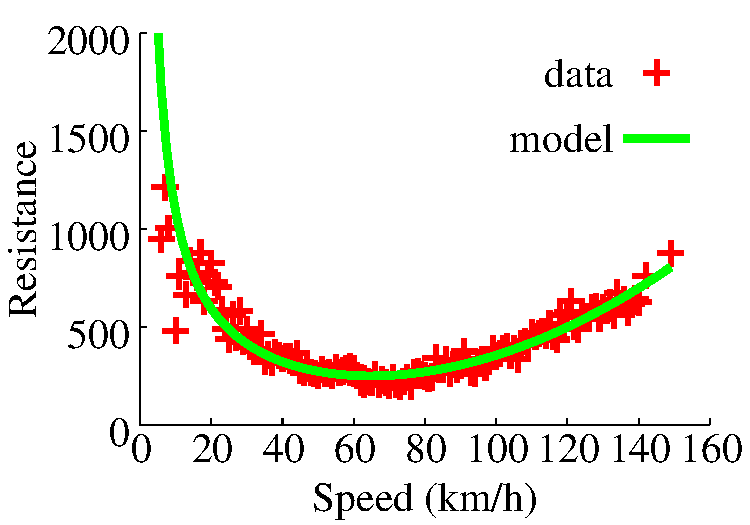
\includegraphics[width=1.8in,angle=0]{Figs/EcoDrive/lei_loss.pdf}
\hspace{-0.0cm}
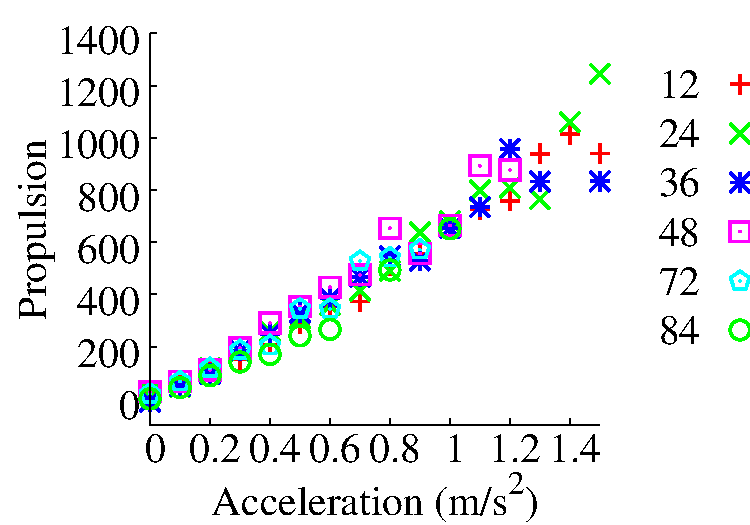
\includegraphics[width=1.8in,angle=0]{Figs/EcoDrive/lei_torque.pdf}
\hspace{-0.0cm}
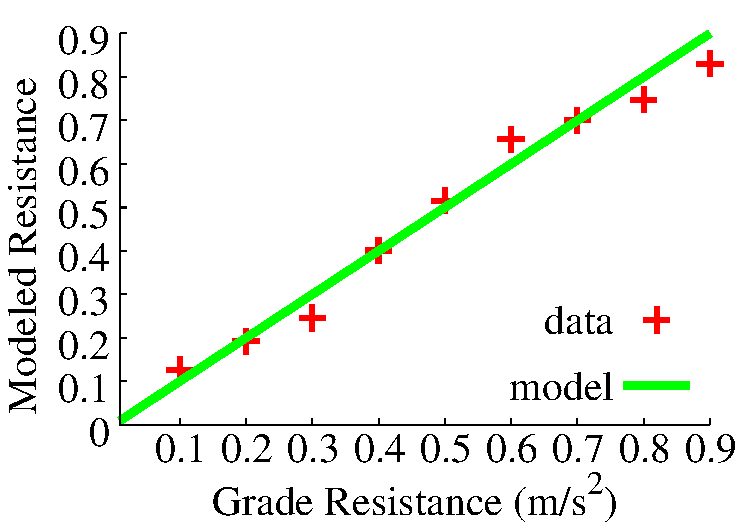
\includegraphics[width=1.8in,angle=0]{Figs/EcoDrive/lei_slope.pdf}
\hspace{-0.0cm}
\vspace{-0.2cm}
\caption{Vehicle Dynamics Modeling. The Figs/EcoDrive are about drivetrain loss and wind resistance under each speed (left), 
relation between acceleration and propulsion (minus wind resistance and drivetrain loss) under each speed (middle), 
modeled grade resistance with groundtruth (right).}
\vspace{-0.8cm}
\label{modeling}
\end{center}
\end{figure*}

\subsection{Propulsion Modeling}


The propulsion (or output torque) of vehicle is closely related
to transmission gear ratios and engine torque \cite{vong2006prediction, giannelli2005heavy}. 
The propulsion produced by vehicle engine
can be represented by

\begin{equation}
 F_p = a_p * \tau_e * R_G.
\end{equation}

where $\tau_e$ refers to the engine torque, 
$R_G$ refers to transmission gear ratio
and $a_p$ is the coefficient used for unit conversion. 


\subsubsection{Gear Ratio Modeling}

Modern vehicles are usually using automatic transmission and 
freeing the driver from shifting gears manually. 
There are mainly two types of transmissions, 
Step Automatic Transmission (SAT) and Continuously Variable Transmission (CVT). 
SAT uses discrete transmission gear ratios while CVT has an
infinite number of effective transmission gear ratios. 
Since different transmission types show different
properties of gear ratio changes over different speeds, 
we use gear ratio changes to identify different
vehicle transmission types. 
We estimate gear ratios by using RPM and speeds 
when the car is driving in constant speeds. 



In a SAT vehicle, $R_G$ are discrete values.
  
\begin{equation}
   R_G = R_i = \frac{RPM}{v}  \hspace{1cm} i = 1,...,n
 \end{equation}

where $v$ represents the vehicular speed 
and $n$ is the number of gears of a transmission, 
e.g., $n=4$ for a 4-speed transmission. 

In a CVT vehicle, $R_G$ changes continuously over time and always
approach the optimal $RPM$. 

\begin{equation}
   R_G =
   \begin{cases}
   \frac{RPM_a}{v}     &  \mbox{if} \hspace{0.2cm} v < v_T, \\
   R_b   &  \mbox{if} \hspace{0.2cm} v \geq v_T.
   \end{cases}
  \end{equation}

where $RPM_a$ is the optimal $RPM$ of a given engine, 
and $v_T$ is the speed threshold. 
If the vehicular speed is lower than $v_T$, 
the engine $RPM$ converges to a constant value $RPM_a$ under
different speeds. 
If the vehicular speed is higher than or equal to $v_T$, 
the gear ratio is a constant value $R_b$. 


\subsubsection{Engine Torque Modeling}


\nop{
\begin{figure}[t]
\begin{center}
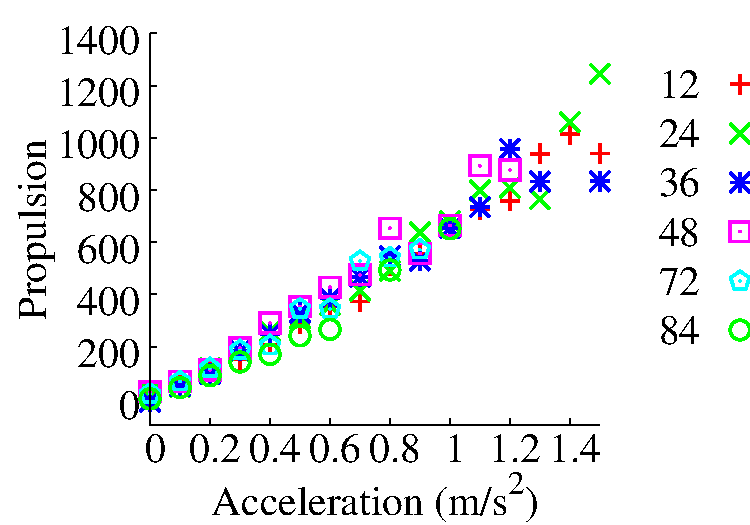
\includegraphics[width=3.0in,angle=0]{Figs/EcoDrive/lei_torque.pdf}
\vspace{-1.0cm}
\caption{Propulsion (output torque) under different speeds (km/h)
and accelerations.}
\vspace{-0.3cm}
\label{speed_propulsion}
\end{center}
\end{figure}
}

Engine torque is produced by the explosion of air and fuel, 
therefore, we can use AFR to model engine torque. 

\begin{equation}
\tau_e = AFR^{f(v)}.
\end{equation}


where $f(v)$ is a parameter function that is monotonically increasing
with vehicular speed. Based on our empirical observation, 
it starts from 0.3 at speed 0 and converges to 1 when the speed
is larger than $20km/h$. 

Therefore, the propulsion of a car on the wheel can be written as 

\begin{equation}
 F_p = a_p * \tau_e * R_G = a_p \frac{AFR^{f(v)} * RPM}{v}.
\end{equation}



\subsection{Drivetrain Loss and Wind Resistance Modeling}

\nop{
\begin{figure}[t]
\begin{center}
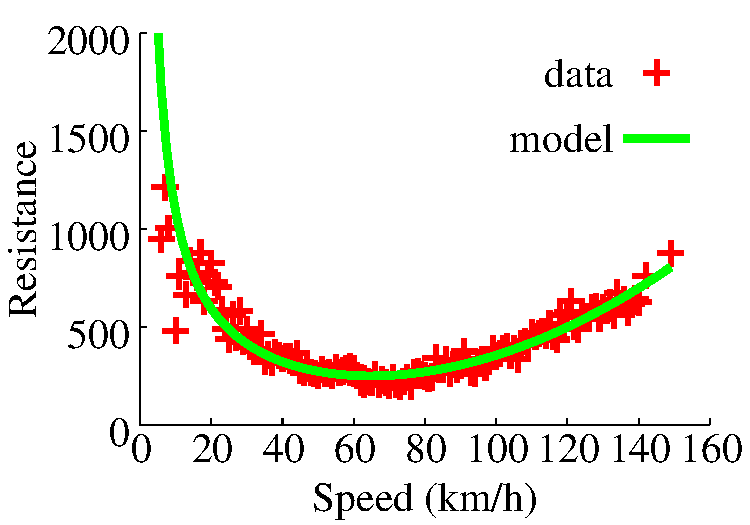
\includegraphics[width=2.4in,angle=0]{Figs/EcoDrive/lei_loss.pdf}
\vspace{-0.3cm}
\caption{Drivetrain loss and wind resistance under different speeds.}
\vspace{-0.3cm}
\label{speed_loss}
\end{center}
\end{figure}
}

Instead of modeling each loss individually, we model all the power losses
as a whole. 
There are mainly two power losses in automotive systems, 
drivetrain loss and wind resistance. 
Drivetrain loss consists of transmission loss and other mechanical system losses.  
Transmission connects car engine and wheels by various gears and
power loss occurs when transmit the power from engine to wheels. 
We model drivetrain loss in the following form.

\begin{equation}
F_l = \frac{a_l}{v} + b_l * v + c_l. 
\end{equation}

where $v$ is the vehicular speed and the rest are coefficients. 
The drivetrain loss drops to minimum when the car is driving
in moderate speed. 


The force from the air drag \cite{andersson2012online} 
can be represented by following equation,

\begin{equation}
 F_w = 0.5 * \rho_a * c_d * A_a * v^2 = a_w * v^2.
\end{equation}

where $\rho_a$ is the air mass density, 
$c_d$ is the air drag coefficient and 
$A_a$ is the effective area of the vehicle. 
Since the effective area of vehicle is different
from vehicle to vehicle, 
we model air drag as a function of vehicle speed
with unknown coefficient $a_w$. 


After we put drivetrain loss and wind resistance together, 
the modeled loss and actual loss are shown in the Fig. \ref{modeling}. 
In low speed, the main loss comes from drivetrain loss due
to mechanical frictions. 
In high speed, the main loss comes from wind resistance due to air compression. 
After we have drivetrain loss and wind resistance, 
we use propulsion minus the loss ($F_p - F_l - F_w$) to model the relation
between acceleration and propulsion, as shown in the middle of Fig. \ref{modeling}. 
For accelerations, we use extra $MAF$ instead of raw $MAF$ readings from 
the OBD port. 
Raw $MAF$ minus the $MAF$ required to maintain a certain speed is
the extra $MAF$ for this speed. 

\subsection{Grade Resistance Modeling}


\nop{
\begin{figure}[t]
\begin{center}
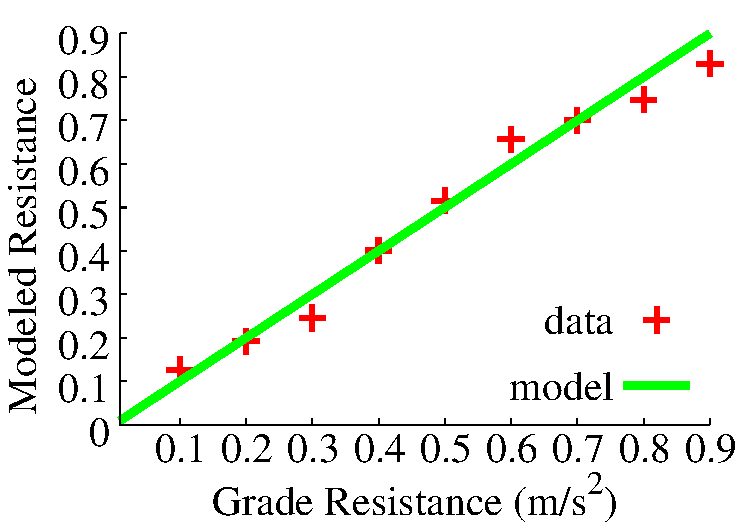
\includegraphics[width=2.5in,angle=0]{Figs/EcoDrive/lei_slope.pdf}
\vspace{-0.3cm}
\caption{Grade resistance.}
\vspace{-0.3cm}
\label{grade_resistance}
\end{center}
\end{figure}
}

Different road types, i.e., flat road, uphill and downhill, 
have significant different impacts on vehicle movements and
fuel consumptions. 
Similar to \cite{andersson2012online}, 
the grade resistance can be modeled as a combination
of forces caused by grade and rolling resistance.
\nop{
Since rolling resistance is a linear function of speed, 
so we combine it with wind resistance and focus on
grade resistance only. 
}
\begin{equation}
    F_r = mgc_r\cos{\theta}.
 \end{equation}
 
where $c_r$ is the grade resistance coefficient, 
$m$ is the vehicle mass, $g$ is the gravity of earth
, $\theta$ is the road grade and $v$ is vehicular speed.
The road elevation information is obtained from
National Elevation Dataset \cite{nationalelevation}. 
\nop{
The dataset provides fine-grained GPS elevation.
We compared the elevation dataset with Google Elevation
API \cite{googleelevation} on some routes,
and the results show that both datasets show similar accuracy. 
}




\subsection{AFR Profile}

Vehicle needs different air/fuel injection rate to achieve
different accelerations under different speeds. 
Based on the vehicle dynamics models we built in 
previous sections, we can build a fuel consumption profile. 
In this profile, we can lookup the AFR required to accelerate
a vehicle with an arbitrary acceleration under any speed. 
Let $AFR(v, a)$ denotes the air/fuel rate is required to 
accelerate the vehicle at acceleration $a$ when the vehicle
is driving at speed $v$. 
The profile can be represented as the following equation. 


\begin{equation}
AFR(v, a) = e^{\frac{log(a/R_G)}{f(v)}} + AFR_c(v)
\end{equation}


\begin{figure}[!htbp]
\begin{center}
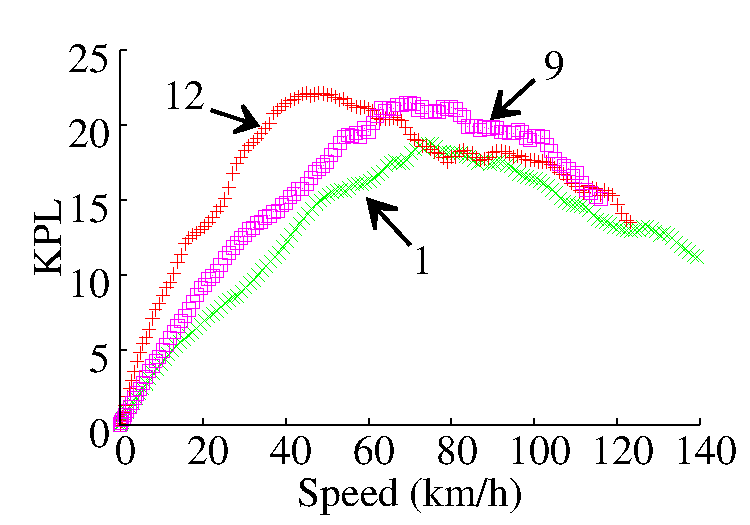
\includegraphics[width=3.0in,angle=0]{Figs/EcoDrive/speed_kpl.pdf}
\hspace{-0.4cm}
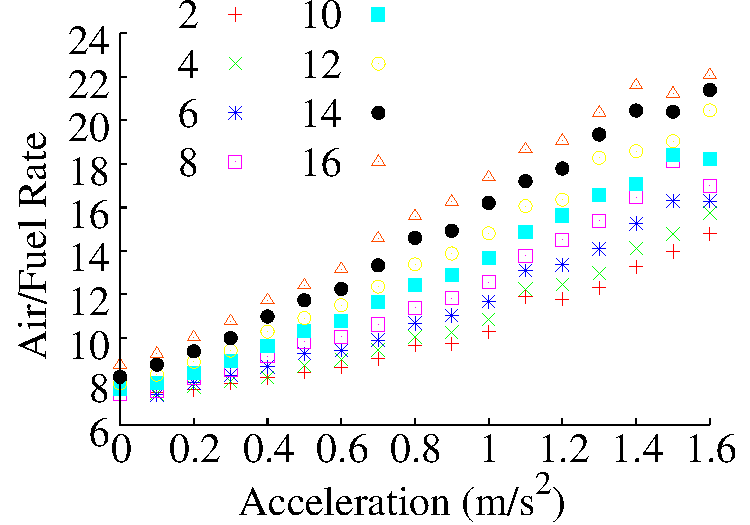
\includegraphics[width=3.0in,angle=0]{Figs/EcoDrive/acce_afr.pdf}
\hspace{-0.4cm}
\vspace{-0.3cm}
\caption{AFR profile.}
\vspace{-0.5cm}
\label{profile}
\end{center}
\end{figure}

An illustration of AFR profile of car 1 is shown in
the right subfigure of Fig. \ref{profile}. 
The profile provides the AFR required to accelerate the car
at a certain acceleration under a certain speed. 
We can infer a lookup table for each $AFR(v, a)$ based
on the profile. 
The left subfigure in Fig. \ref{profile} illustrates different
vehicles have different speed-KPL matching, 
which indicates AFR profile needs to be built
based on individual vehicles. 




 







\section{Acceleration Control}



EcoDrive controls air/fuel injection rate to control vehicular speed 
by emulating gas pedal. 
EocDrive calculates accelerations of each speed and leaves
brake decision to drivers or other systems. 
It needs two inputs, road speed limit and segment length. 
The speed limit can be set by human drivers or queried from online database \cite{speedlimit}. 
The road segment length can be estimated by human drivers or
by a third-party navigation software. 
Road segment length is not necessary for long distance roads, 
as the driving strategy will be the same if the distance is longer than
a threshold.
For example, if the speed limit is $25mph$, 
the fuel efficient acceleration strategies for $300m$ and $500m$ are the same. 
We assume both speed limit and road segment length are known. 
The output of EcoDrive is a matrix and each element in the matrix is the minimum
fuel consumption when the car arrives at a certain distance with a certain speed. 
By traversing all the possibilities, EcoDrive is able to find all reasonable
driving strategies with different fuel consumption and travel time. 


\subsection{Problem Statement}

Driving pattern can be abstracted as accelerate-cruise-brake.  
EcoDrive focuses on the accelerate-cruise part and 
leaves brake decision to human drivers. 
For example, in a $300m$ road segment with speed limit $25mph$ (or $40km/h$), 
the EcoDrive accelerates and cruises to $200m$ and 
the driver uses the rest $100m$ to stop the car as
there is a stop sign at the end of the road. 
Similar to cruise control, we assume there is enough distance
to front obstacles for drivers to brake.


EcoDrive needs two key inputs: 1) The length of the road segment, 
i.e., from current location to the point driver will make a brake, 
2) The lower and upper speed limits of the road segment. 
Such inputs can be given by user or extracted from online databases and navigation
softwares.
We focus on how to utilize such inputs to calculate
fuel efficient strategies.  
Therefore, the problem that EcoDrive is going to address can
be stated as follows:
\emph{Given a road segment length with lower and upper speed limits,
how to control air/fuel injection rate in real time to achieve the most fuel efficient driving strategy}.  


\subsection{Driving Strategy by Dynamic Programming}


\nop{
\begin{table*}[t]
        \centering
        \caption[symbols]{Notations used calculate fuel efficient driving strategy}
         \vspace{0.5cm}
        \label{symbols}
                \begin{tabular}{|l|l|}
                \hline
Symbol & Meaning 
\\  \hline      \hline
$v_i$ & The $i$th speed of the vehicle  
\\  \hline 
$a_j$ & The $j$th acceleration of a given speed 
\\  \hline
$D$ & The travel distance of the road  
\\  \hline
$d_k$ & The $k$th road segment, $D = \sum{d_k}$      
\\  \hline
$s(i, k)$ & A state represents that the car is driving 
          in speed $v_i$ at the start location of segment $d_k$ 
\\  \hline
$FC(i, k)$ & The fuel consumption that the car can reach
          state $s(i, k)$
\\  \hline
$AFR(v_i, a_j)$ & The air/fuel rate if the car is 
     driving at speed $v_i$ with acceleration $a_j$
\\  \hline
      \end{tabular}
\end{table*}
}

We use dynamic programming to traverse all the possibilities 
to find all reasonable driving strategies. 
This is inspired by the fact that the fuel efficiency and travel
time are related to the speed and distance. 
We divided the road segment into smaller equal length
road segments.  
We use $v_i$ and $d_k$ to represent the $i$th speed 
and the length of $k$th segment, respectively. 
%A detailed notation table is shown in Table \ref{symbols}. 
We use $s(i, k)$ to represent the state when the car is driving
at speed $v_i$ at the start location of road segment $d_k$. 
For any state $s(i, k)$, there are two sets of possible transitions. 
First, it transits from $s(i, k - 1)$, which means that the
car is driving in constant speed $v_i$ in last road segment. 
Second, it transits from $s(i - 1, k - 1 - m)$, 
which means the car is accelerating from speed $v_{i - 1}$ to $v_i$
under acceleration $a_j$. The lower speed bound is used to eliminate
some unreasonable cruising speed, e.g. it is obviously not fuel efficient and 
reasonable if the car is cruising at 1 km/h.    

In the first case, the accumulated fuel consumption is the sum
of the fuel consumption used to reach state $s(i, k - 1)$ and 
the cruising fuel consumption from $d_{k - 1}$ to $d_k$. 
\begin{equation}
FC_c(i, k) = FC(i, k - 1) + AFR(v_i, 0.0) * t_i. 
\end{equation}

where $t_i$ means the time cost when the car is driving
through road segment $d_{k - 1}$
and $t_i = \frac{d_{k - 1}}{v_i - v_{i - 1}}$. 


In the second case, the accumulated fuel consumption 
is the sum of the fuel consumption used to reach 
state $s(i - 1, k - 1 - m)$, the cruising fuel consumption 
$FC_c$ in part of road segment $k - 1 - m$, 
and the acceleration fuel consumption $FC_j$. 
The car may start to accelerate at any location in 
road segment $k - 1 - m$.  
The road segment is split into two parts, 
the car cruises to a point within the road segment
$k - 1 - m$ and then starts to accelerate at 
acceleration $a_j$. 
Therefore, the fuel consumption of this case can
be represented as follows. 

\begin{equation}
FC_a(i, k) = FC(i, k - 1 - m) + FC_c + FC_j. 
\end{equation}


where $FC_c = AFR(v_i, 0.0) * t_c$ and $t_c$ is
the cruising time cost within road segment $k - 1 - m$.
To calculate $t_c$, we need to calculate the distance
used to accelerate from $v_{i - 1}$ to $v_{i}$. 
Before that, we present 
the acceleration fuel consumption cost as
\begin{equation}
FC_j = AFR(v_{i - 1}, a_j) * t_a. 
\end{equation}

The acceleration time is $t_a = \frac{v_i - v_{i - 1}}{a_j}$ and
the acceleration distance is $d_a = v_{i - 1} * t_a + 0.5 * a_j * t_a^2$. 
The cruising distance is simply $d_c = \sum_{x = k - m - 1}^{k - 1}{d_x} - d_a$
and the cruising time is $t_c = \frac{d_c}{v_{i - 1}}$. 


Therefore, the fuel consumption at the start of state $s(i, k)$ is

\begin{equation}
FC(i, k) = min\{FC_c(i, k), min\{FC_a(i, k)\}\}. 
\end{equation}

After we traverse all the states, the last state of each speed
is the minimum fuel consumption when the car is finally cruising
in that speed. The most economy driving strategy can be traced
back from the state with minimum fuel consumption. 
Different travel time is used when the car is cruising in 
different speeds. 
By using this property, we can find a tradeoff between travel
time and fuel consumption. 


Assume that we split the road segment into $n$ smaller equal length road segments
, there are $m$ different speeds and $l$ different accelerations, 
the time complexity of the dynamic programming algorithm is $O(n*m*l)$
and the space complexity is $O(n * m)$. 
In practice, the most road segment length in urban area is less than $1km$
and we set each smaller road segment to be $1m$. 
The unit of the speed sensed from the OBD port is $km/h$ and the speeds are
integers, so we have $0-60$ different speeds in 
urban area. 
The acceleration is normally from $0.1m/s^2$ to $1.4m/s^2$. 
Therefore, the time complexity of the algorithm grows linearly 
with the total road length. 


Different road conditions affect air/fuel rate as the car needs
lower (or higher) air/fuel injection rate to achieve the same acceleration
in downhill (or uphill) conditions.  
The air/fuel rate for a specific road segment $d_k$ becomes $AFR(v_i, a_j - a_k)$, 
where $a_k$ refers to the acceleration/deceleration caused by the $k$th road segment. 
The driving strategy can be calculated based on the dynamic programming solution as well.  

\subsection{Fuel Economy and Travel Time}


In general, fuel efficient driving
strategies require longer travel time in urban environments. 
Therefore, there is a trade-off between fuel efficiency 
and travel time. 
EcoDrive provides different travel time by selecting different
target speed. 
The higher the target speed, the less the travel time. 
The user can select the most fuel efficient driving
strategy with fixed target speed, 
or select desired travel time with corresponding target speed. 
The selection of target speed also depends on the speed limit,
i.e., the target speed should not be higher than the speed limit. 
The most fuel efficient cruising speed ranges from 30mph to 60mph
for different types of vehicles. 
In urban environments, the most fuel efficient target speed
is around the speed limit. 
However, in short road segments, it is generally more fuel efficient to
select a target speed that is lower than speed limit 
due to extra cost on acceleration. 



\subsection{Highway Strategy}

The most fuel efficient highway speeds range from $40km/h$ to $80km/h$ 
for the vehicles we observed.  
Given the highway speed limit ranging from $80km/h$ to $110km/h$ in US, 
drivers can find a trade-off between fuel efficiency and travel time
by selecting different cruising speeds. 
Generally speaking, constant speed cruising generally has higher KPL
than frequent accelerations and decelerations. 
Therefore, traditional cruise control is considered a good option for economic driving. 
However, traditional cruise control sticks to one target speed. 
If the driver manually increases target speed, the car will aggressively 
approach to the target speed, which will bring extra fuel consumptions. 
Similarly, when the car is cruising uphill, the road will slow down
the car and cruise control will aggressively approach the target speed. 
In downhill condition, cruise control will reduce air/fuel injection
to maintain the target speed. 
EcoDrive increases speed gradually and utilizes the acceleration caused by downhill
to achieve higher KPL.  



\subsection{Acceleration Controller}


\begin{figure}[t]
\begin{center}
\vspace{-0.2cm}
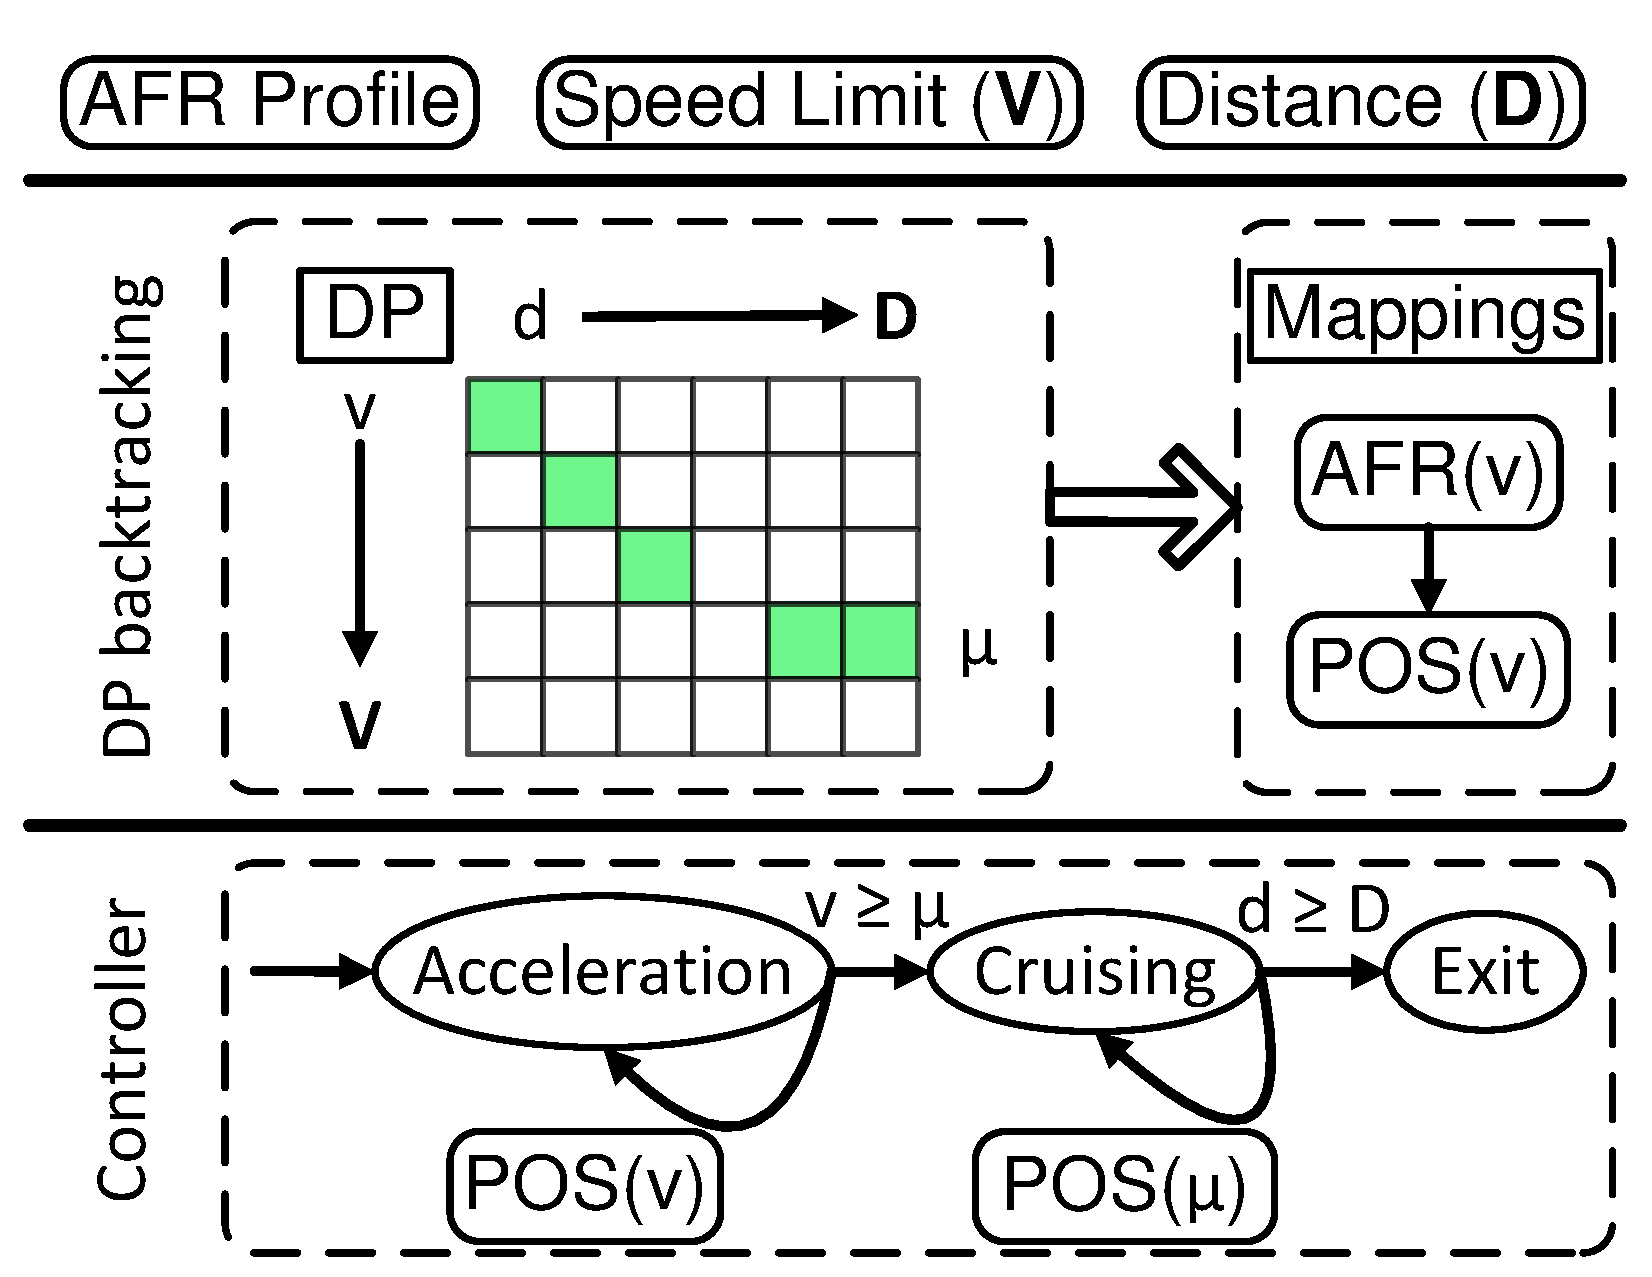
\includegraphics[width=4.0in,angle=0]{Figs/EcoDrive/controlflow.pdf}
\vspace{-0.0cm}
\caption{EcoDrive control flow.}
\vspace{-0.5cm}
\label{controlflow}
\end{center}
\end{figure}



We summarize the control flow of EcoDrive in Fig. \ref{controlflow}. 
The AFR profile is calculated offline by the modeling component. 
Given the travel distance $D$ and speed limit $V$, 
EcoDrive uses dynamic programming model to calculate the speed
to acceleration mapping of the most economic driving strategy. 
This process is done by backtracking the last state of target speed $\mu$. 
The speed to acceleration mapping records the desired
acceleration under that speed. 
This mapping is converted into speed to air/fuel injection rate
mapping $AFR(v)$ by querying the AFR profile. 
The acceleration controller retrieves the air/fuel injection
rate based on the mapping and real-time sensed vehicular speed. 
A air/fuel rate to gas pedal position mapping and 
a gas pedal position to voltage mapping are calculated in advance.
The controller gets the speed to gas pedal position mapping $POS(v)$.  
Based on the air/fuel injection rate, EcoDrive sends 
corresponding voltage values to the ECU. 
In this process, EcoDrive maintains three states, 
acceleration, cruising and exit. 
EcoDrive is in acceleration state by default and enters
cruising state when sensed OBD speed is not less than target speed. 
After it enters cruising state, it remains constant air/fuel
rate injection. 
Different from traditional cruising control, 
EcoDrive may increase/decrease speed in cruising state
by adapting to various road conditions. 
If the car reaches the distance or EcoDrive is turned off
by switch of brake, it enters exit state. 
EcoDrive releases all the resources in exit state
and aborts to wait for next inputs. 




\section{In-vehicle Setup and Implementation}


We explain the in-vehicle setup and implementation of EcoDrive.


\subsection{In-vehicle Setup}


\begin{figure}[t]
\begin{center}
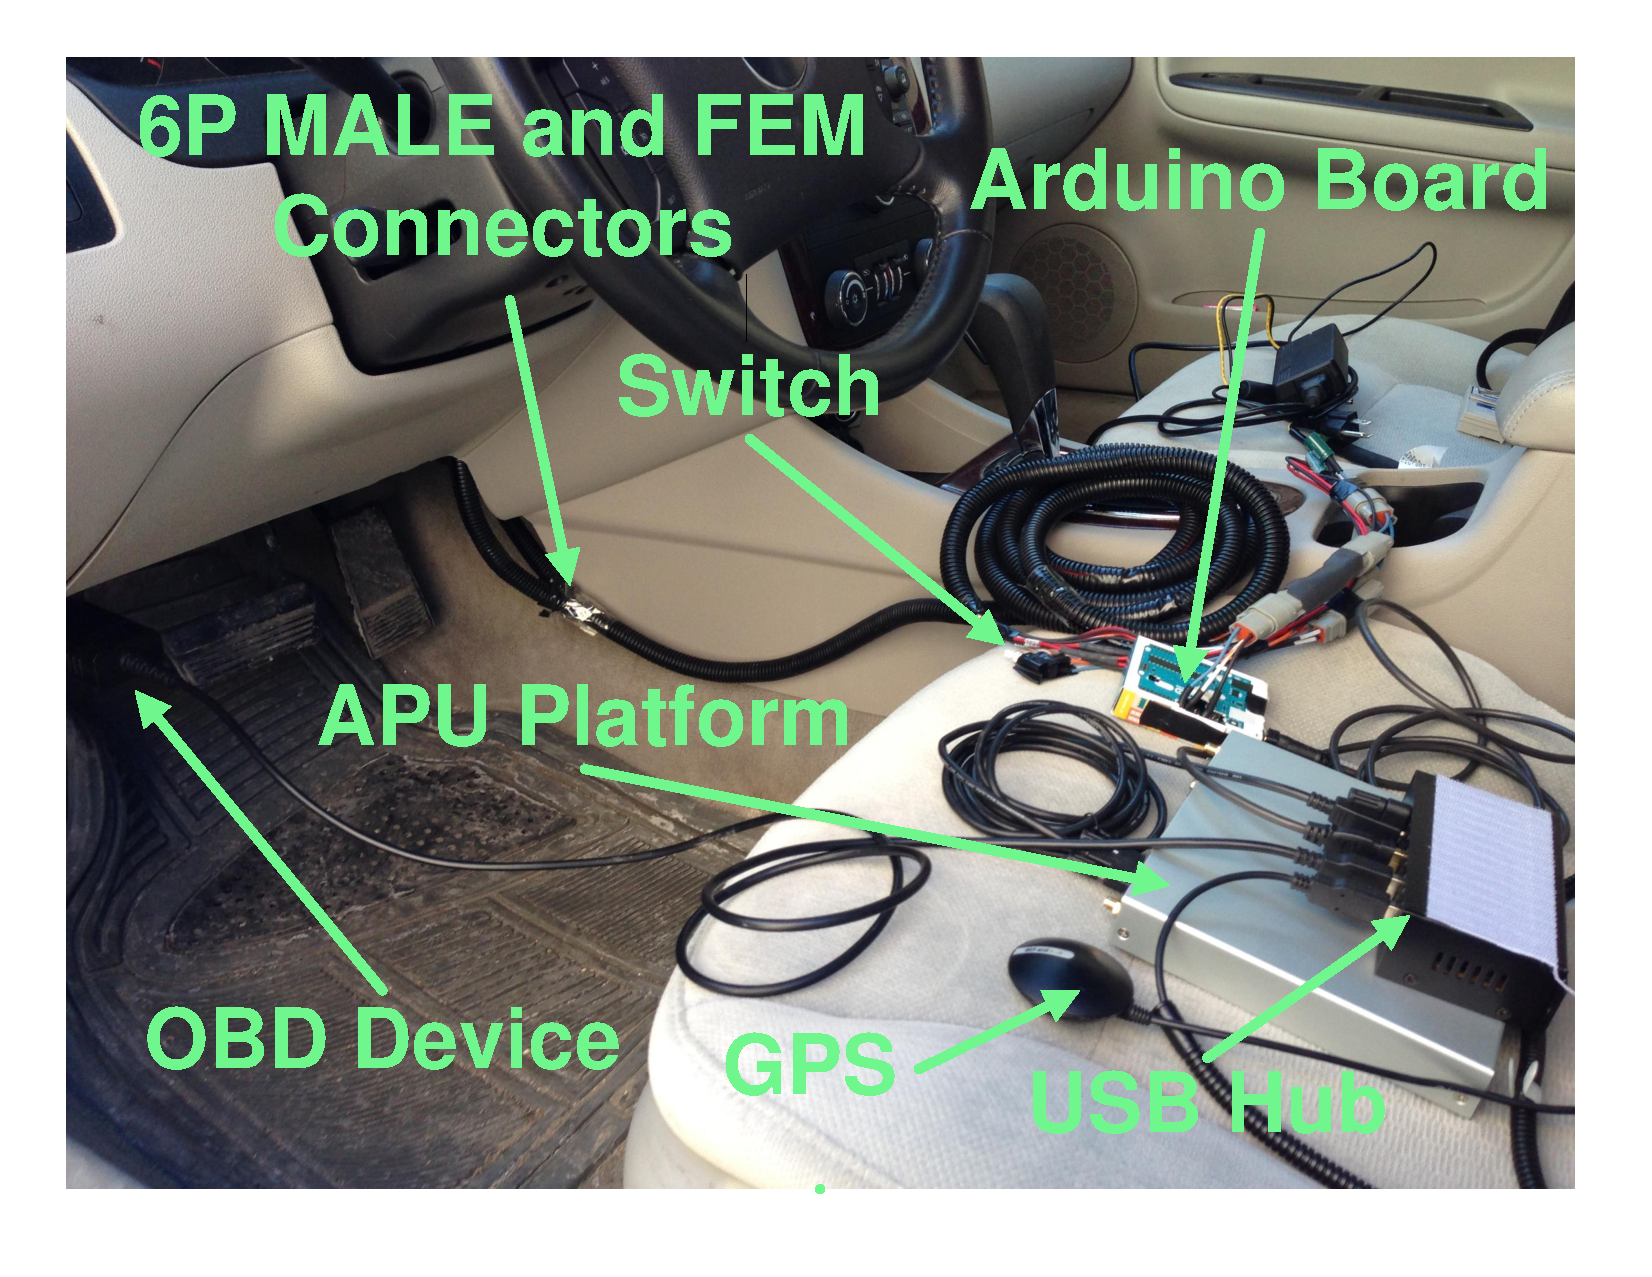
\includegraphics[width=3.0in,angle=0]{Figs/EcoDrive/setup_3.pdf}
\vspace{-0.3cm}
\caption{EcoDrive in-vehicle setup.}
\vspace{-0.6cm}
\label{setup}
\end{center}
\end{figure}


The in-vehicle setup of EcoDrive is shown in Fig. \ref{setup}. 
EcoDrive uses Arduino Uno microcontroller to emulate 
gas pedal by delivering signals to the ECU through a 6P FEM Connector. 
The microcontroller outputs a 16-bit resolution digital pulse-width modulation (PWM) 
signal which is smoothed out by an RC filter. 
A 6P MALE Connector is used to read signal outputs from 
the original gas pedal. 
A wiring harness and switch button are built that allows the user 
to switch the signal read by the ECU between the gas pedal and 
the microcontroller.  
Therefore, the setup supports two mode, human driving mode and
EcoDrive mode. 
In human driving mode, the gas pedal and air/fuel injection rate
is controlled by human driver.
In EcoDrive mode, the gas pedal is unusable and air/fuel injection rate
is controlled by the system. 
In EcoDrive mode, The APU platform \cite{apu} sends pedal positions to the microcontroller through 
serial communication and the microcontroller converts the pedal position values 
into analog voltages outputs. 
To do this, we construct a mapping between sensor analog 
voltage outputs and pedal positions. 
By using the mapping between gas pedal position
and air/fuel rate built from driving traces, 
we can send position values from laptop to the car
to control air/fuel injection rate.  

\vfill\eject

\subsection{Implementation}


We implement EcoDrive data sensing module and air/fuel
injection control module in C++. 
We operate EcoDrive on the Ubuntu 14.04 32bit distribution 
(with linux kernel version 3.13.0-34-generic), 
that runs on PC Engines APU platform \cite{apu}. 
APU platform is a mobile embedded platform that 
is equipped with 1GHz dual core CPU and 4G DDR3 DRAM. 
EcoDrive uses two threads to
query and read OBD messages, respectively. 
One thread sends OBD query message to the OBD port in every 250ms.
Higher frequency OBD query will cause CAN read error. 
Another thread listens on the OBD port for 
echo messages and sends voltage control commands to 
Arduino board. 
The Arduino board initiates a loop to listen on the USB 
serial and sets the voltage output of two pins 
based on received command. 
The two pins represent the voltage output pins
of gas pedal's two position sensors. 



\nop{
\subsection{OBD Data Collection}


\begin{figure}[!htbp]
\begin{center}
\vspace{-0.0cm}
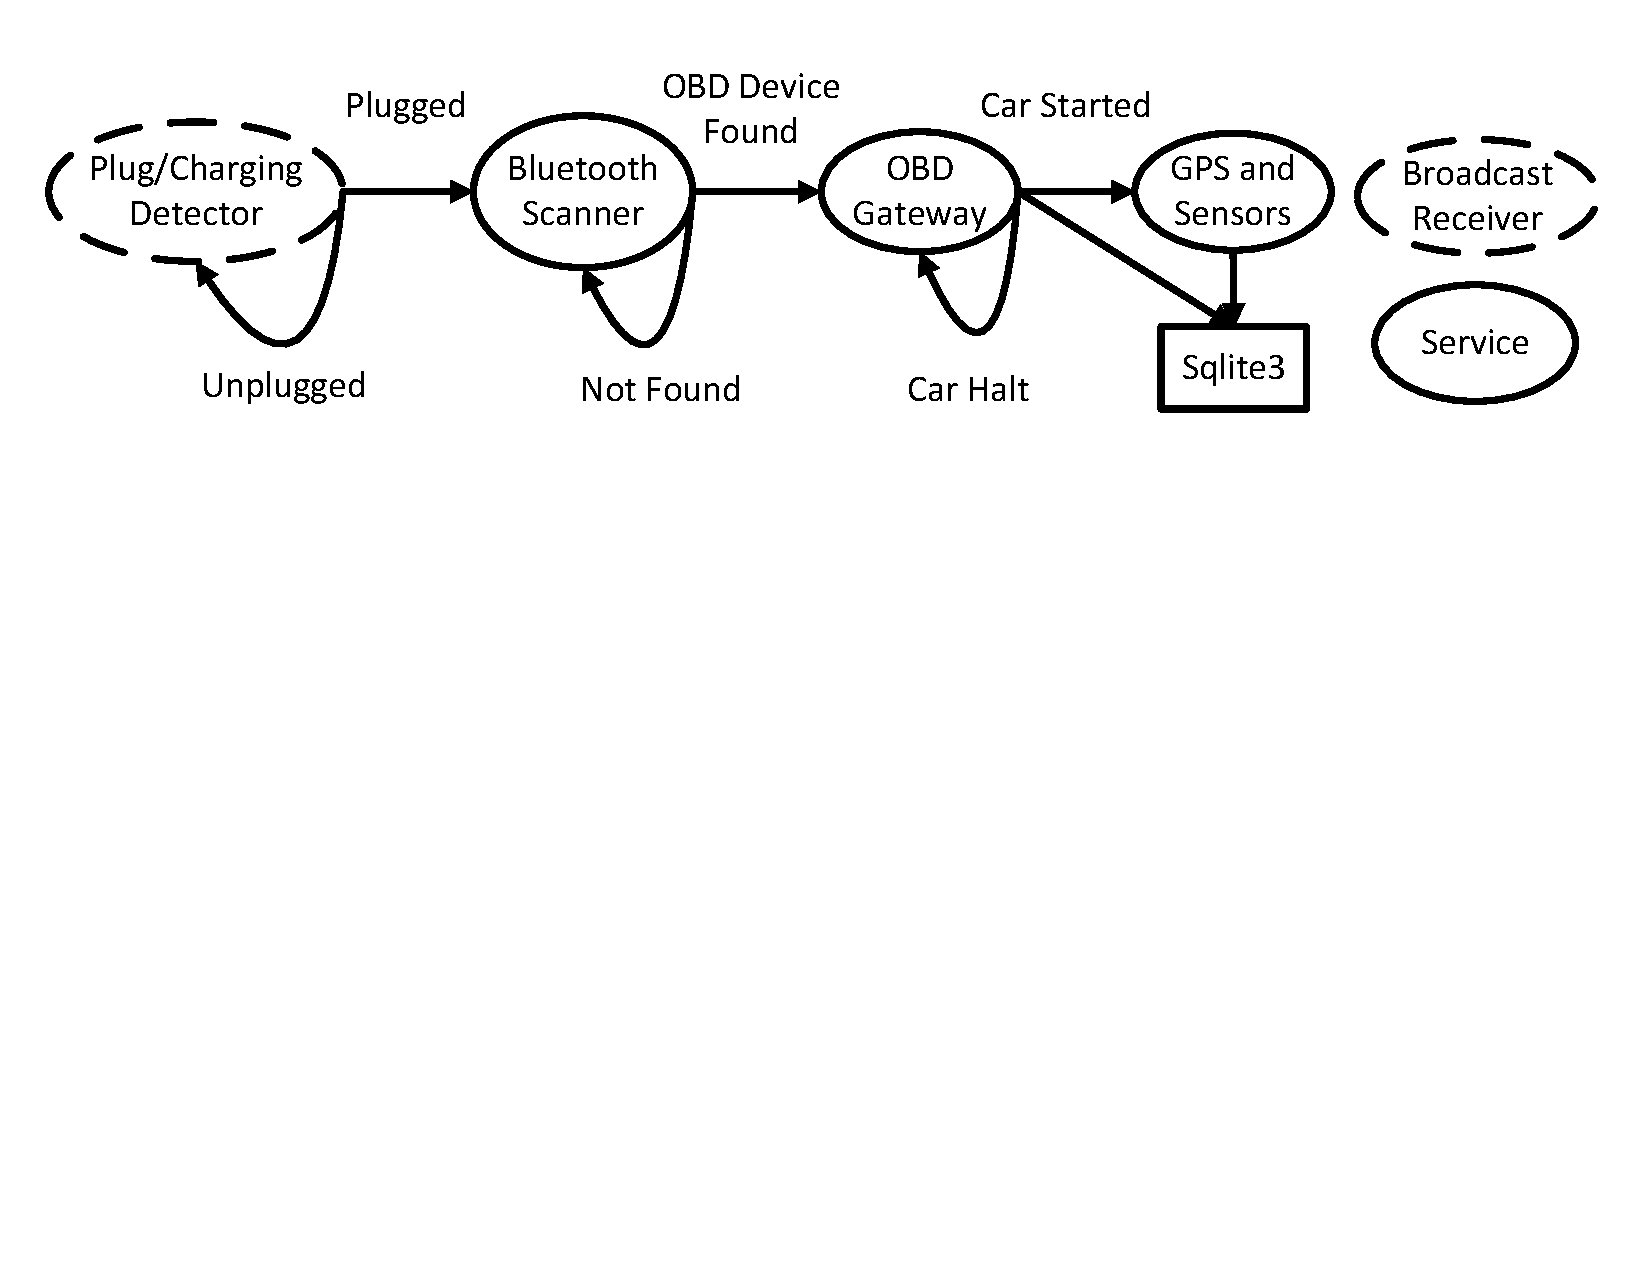
\includegraphics[width=3.0in,angle=0]{Figs/EcoDrive/datacollection.pdf}
\vspace{-5.0cm}
\caption{The control flow of Android application that is used for OBD data collection.}
\vspace{-0.4cm}
\label{data_collection}
\end{center}
\end{figure}

To collect driving data from different vehicles, 
we use Motorola Xoom with customized data collection
Android application.
Motorola Xoom is plugged with car charger adapter
and interacts with a standard bluetooth OBDII scan device. 
The control flow of the application is shown in Fig. \ref{data_collection}. 
In our setting, the tablet car charger adapter is always
plugged into the in-car charger outlet.  
Turning on the ignition will start charging the tablet, 
while some cars can still charge the tablet after car stalls, 
i.e., 2011 Chevrolet Impala, 2005 Buick LaCrosse etc. 
The plug/charging detector is a broadcast receiver to detect
the plug/charging status of the tablet. 
The broadcast receiver reads the charging status of 
the tablet periodically by using \emph{AlarmManager}. 
\emph{AlarmManager} can hold a CPU wake lock to guarantee that 
the tablet will not sleep and the application wakes up periodically.
The Bluetooth Scanner tries to connect to the OBD device. 
Once a bluetooth OBD device is found, 
the OBD Gateway sends OBD messages to test the engine
status of the car.
This is used to deal with the cars that the tablet is still charging
even after turning off the ignition. 
If the car engine is started, the application starts to write
the OBD messages and results into sqlite3 databases.  
GPS and other sensor data from the tablet are also collected. 
Each trip is recorded in a database file. 


}



\section{Experimental Results}


Our evaluation consists of four parts, EcoDrive road testing results in both urban and highway environments, 
vehicle dynamics modeling accuracy, 
driving data statistics and trace-driven simulation. 


\subsection{Fuel Efficiency Test Results}


%\subsubsection{Test Drive Example}

\subsubsection{Urban}

\begin{figure}[!htbp]
\begin{center}
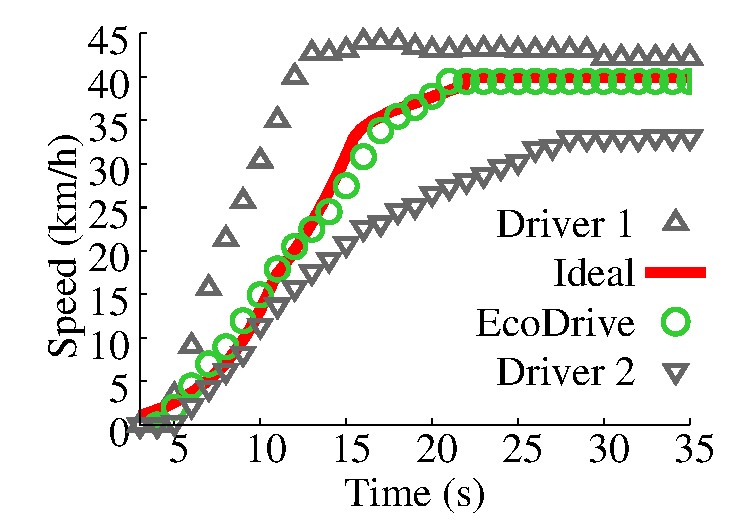
\includegraphics[width=3.0in,angle=0]{Figs/EcoDrive/evaluation/sampledrive240.pdf}
\vspace{-0.0cm}
\caption{Driving behaviors of EcoDrive and Human Drivers on a 300m length road segment.}
\vspace{-0.6cm}
\label{sampledrive}
\end{center}
\end{figure}


In this experiment, we compare EcoDrive with human drivers in urban
road segments.  
EcoDrive uses drive-by-wire technology to control air/fuel injection rate. 
It accelerates the vehicle by sending gas pedal position values to ECU. 
EcoDrive provides driver a switch button which can disable EcoDrive immediately. 
In our evaluation, we did not experience any bugs or out of control situations, 
but we made our risk management as follows. 
First, we control the input parameters. i.e., the gas pedal position value, 
on both the controller and the Arduino board. 
Second, we can shift the transmission to neutral or park to disconnect the engine and wheel
if the engine is out of control due to unexpected gas pedal position input. 
Third, the brake dominates the gas pedal and we can brake
even when the engine is out of control. 



\textbf{Test Drive Example}. 
A EcoDrive prototype test drive and human drive tests are conducted in a $300m$ length
road segment with speed limit of 25mph (or 40km/h). 
The vehicular speed traces are shown in Fig. \ref{sampledrive}. 
The ideal curve is plotted from the traces obtained from dynamic programming model. 
In our prototype, the air/fuel injection rate is controlled based
on sensed speed. 
The speed may change at any point during the query interval, 
so that it is challenge to control the air/fuel injection rate precisely at each speed. 
The differences between estimated speed traces and
actual speed traces are mainly caused by the impreciseness of 
speed sensing and road conditions.  
Some other factors affect the preciseness of vehicular speed 
control include wind speed and passenger
weights etc. 
Two human drivers are asked to drive 
on the same road segment. 
It is shown that the driver 1 is more aggressive by fast accelerations
and driver 2 is more conservative by slow accelerations. 
The driving trace of EcoDrive prototype falls in between. 
In this comparison, the prototype shows 23\% and 19\% fuel
efficiency improvements than driver 1 and 2, respectively. 
Driver can reach a fuel efficient speed faster by fast acceleration, 
but it takes more fuel during the acceleration process.  
If a driver uses lower accelerations to reduce fuel consumption
during acceleration process, overall fuel efficiency will not be increased due to driving in low (less fuel efficient) speeds
and longer travel time.
EcoDrive chooses the best strategy for economic driving. 


%\subsubsection{Urban Road Segments}


\begin{figure}[t]
\begin{center}
\vspace{-0.5cm}
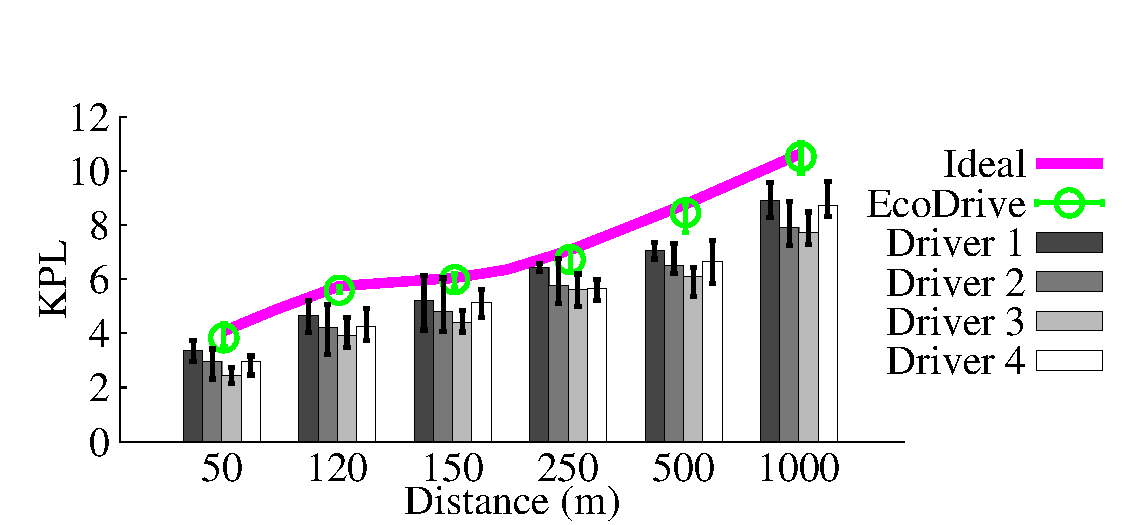
\includegraphics[width=3.0in,angle=0]{Figs/EcoDrive/evaluation/urbansegments.pdf}
\vspace{-0.0cm}
\caption{Fuel efficiency comparison between EcoDrive and human drivers on urban road segments. }
\vspace{-0.7cm}
\label{urbansegments}
\end{center}
\end{figure}

\textbf{Urban Road Segments}. 
We select six different road segments and let EcoDrive drive the car 10 times on each road segment. 
We recruited four drivers to drive on the same
road segments 10 times as well. 
The speed limit of the $500m$ and $1000m$ road segments
is $30mph$ (or $50km/h$) and the that of the $150m$
and $250m$ road segments is $25mph$ (or $40km/h$). 
There is no speed limit for the $50m$ and $120m$ road segments.
The length is the driving length of EcoDrive and 
the overall road segment length is longer so
that drivers have enough time to stop the car. 
The results are shown in Fig. \ref{urbansegments}. 
The ideal fuel consumption is the theoretical 
fuel consumption that is calculated based on AFR profile and dynamic programming model. 
The actual fuel consumption of EcoDrive on certain
road segment length is very stable. 
EcoDrive shows 10\%-40\% fuel efficiency improvement 
compared to different drivers with different road segment lengths. 
The fuel efficiency improvement comes from the smooth driving behaviors of EcoDrive. 
EcoDrive has an average of 20\% more travel time than human drivers.  
EcoDrive can have 5\%-10\% improvements than human drivers if not sacrificing travel time.
The plots of tradeoff between fuel consumption and travel time
are omitted due to the space limit. 

\subsubsection{Highway}


In this experiment, we compare EcoDrive with cruise control and human drivers
on highway. 

\begin{figure}[!htbp]
\begin{center}
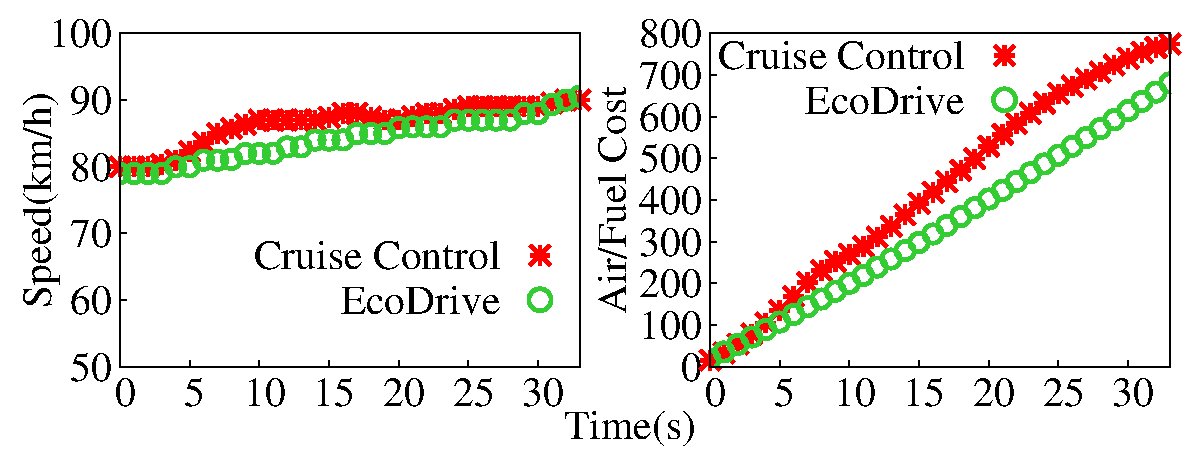
\includegraphics[width=5.0in,angle=0]{Figs/EcoDrive/evaluation/cruise_ecodrive_compare.pdf}
\vspace{-0.0cm}
\caption{Acceleration comparison between Cruise Control and EcoDrive. }
\vspace{-0.4cm}
\label{cruiseecodrive}
\end{center}
\end{figure}


\textbf{Compare to Cruise Control}. 
Fig. \ref{cruiseecodrive} plots the different acceleration patterns between cruise control
and EcoDrive. 
Cruise control is a vehicle built-in feature that can keep car driving
at a certain speed while human drivers can manually increase or decrease the cruising speed. 
The cruise control pattern is extracted when the gas pedal position is 0 but 
the air/fuel injection rate is higher than the idle state rate.  
As shown in the figure, cruise control consumes more
fuels than EcoDrive due to the aggressive acceleration strategy. 
The travel distance is similar for both cases, so EcoDrive is more fuel
efficient than cruise control. 
Similarly, driving uphill by using cruise control will consume more fuels as well. 
When the car is driving uphill, the vehicular speed drops due to grade resistance,
so cruise control will aggressively accelerate to the setting speed. 
In downhill conditions, cruise control will reduce air/fuel injection rate, 
while accelerating by maintaining the same air/fuel injection
rate has higher fuel efficiency. 


\begin{figure}[!htbp]
\begin{center}
\vspace{-0.4cm}
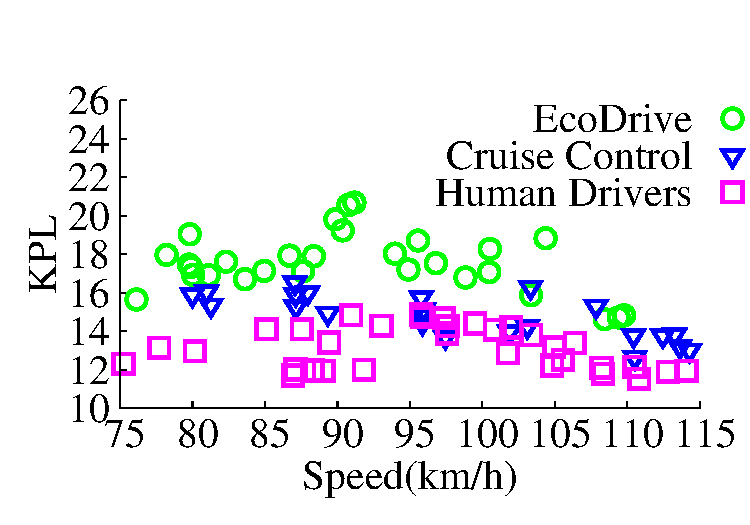
\includegraphics[width=3.0in,angle=0]{Figs/EcoDrive/evaluation/highway_ecodrive.pdf}
\vspace{-0.0cm}
\caption{Highway experiments.}
\vspace{-0.6cm}
\label{ecodrive_highway}
\end{center}
\end{figure}


\textbf{Compare to Human Drivers}. 
We evaluate EcoDrive by driving on two highway segments, 
one is a local highway segment and another is a cross state highway segment.  
The highway segments are selected based on historical driving traces of car 1. 
EcoDrive is evaluated by two-way driving in each highway segment, 
e.g., if EcoDrive enters highway at A and exits at B in one experiment
and it will enter at B and exits at A in next experiment.  
The two-way road testing is used to evaluate EcoDrive in both uphill
and downhill conditions. 
EcoDrive is evaluated between exit 256 and 262 on Madison's West Betline Highway, 
and between exit 132 and 136 on US 14 Highway.

The cruise control and human driving traces are extracted from 
historical driving traces collected on the same highway segments. 
In each driving trace, the car is traveling at a
constant speed(it may have some small speed variations). And we calculate the average speed of each trace as the vehicle speed.
The results are shown in Fig. \ref{ecodrive_highway}, where
each point represents the KPL of a $2km-3km$ length road segment. 
To eliminate the impact of traffic, the traces that 
have speed decrease due to brake are not included. 
In this experiment, EcoDrive shows more than 10\% fuel efficiency than cruise control
and more than 30\% fuel efficiency than human drivers on average. 



\subsubsection{Travel Time and Fuel Efficiency}

\nop{
\begin{figure}[!htbp]
\begin{center}
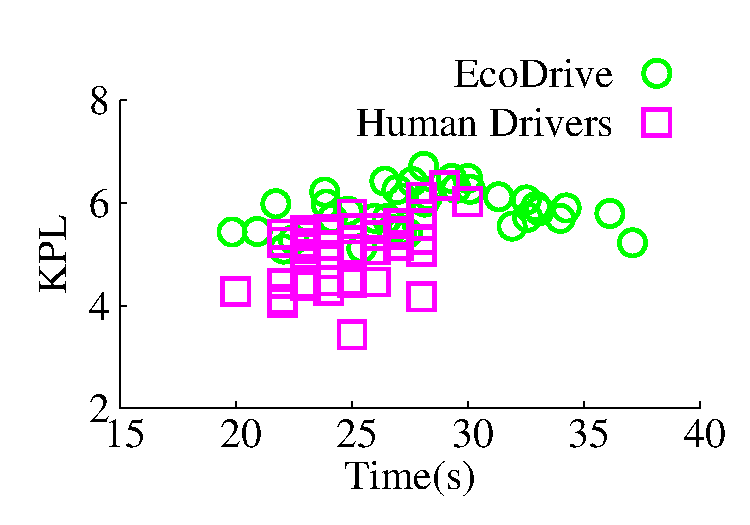
\includegraphics[width=1.7in,angle=0]{Figs/EcoDrive/evaluation/urban_timekpl.pdf}
\hspace{-0.5cm}
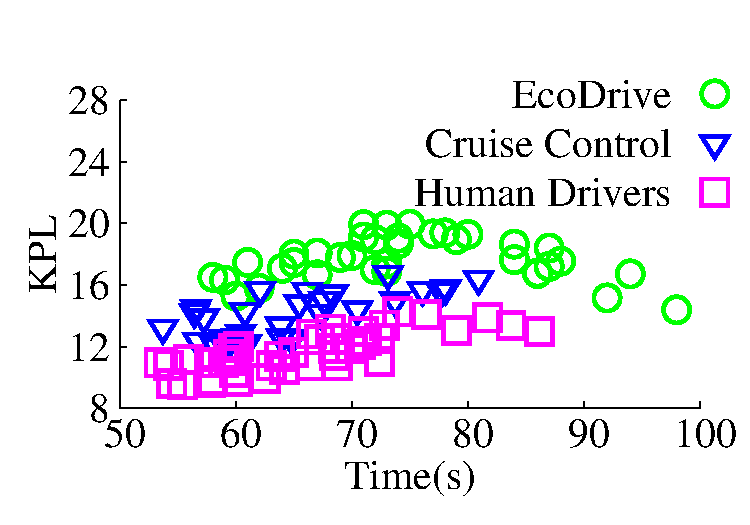
\includegraphics[width=1.7in,angle=0]{Figs/EcoDrive/evaluation/highway_timekpl.pdf}
\vspace{-0.2cm}
\caption{Trade off between travel time and fuel consumption in urban(left) and highway(right) environments.}
\vspace{-0.6cm}
\label{traveltime}
\end{center}
\end{figure}
}

\begin{figure}[!htbp]
\begin{center}
\vspace{-0.4cm}
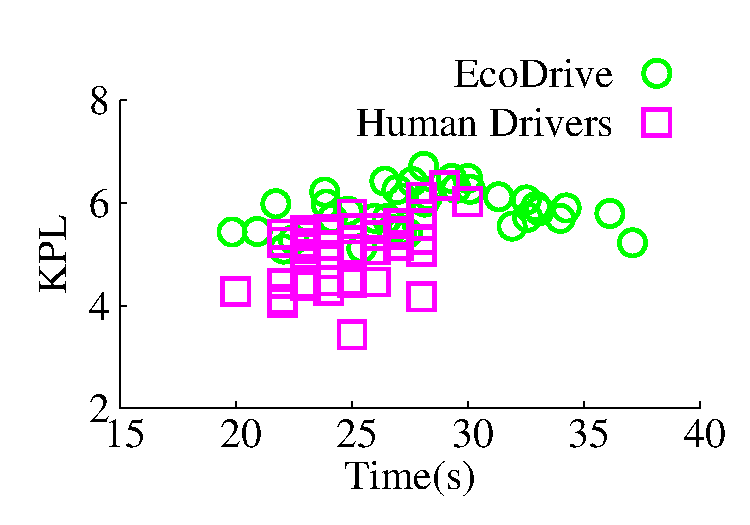
\includegraphics[width=3.0in,angle=0]{Figs/EcoDrive/evaluation/urban_timekpl.pdf}
\vspace{-0.0cm}
\caption{Tradeoff between travel time and fuel consumption on a 250m road segment.}
\vspace{-0.6cm}
\label{tradeoff_urban}
\end{center}
\end{figure}

\begin{figure}[!htbp]
\begin{center}
\vspace{-0.4cm}
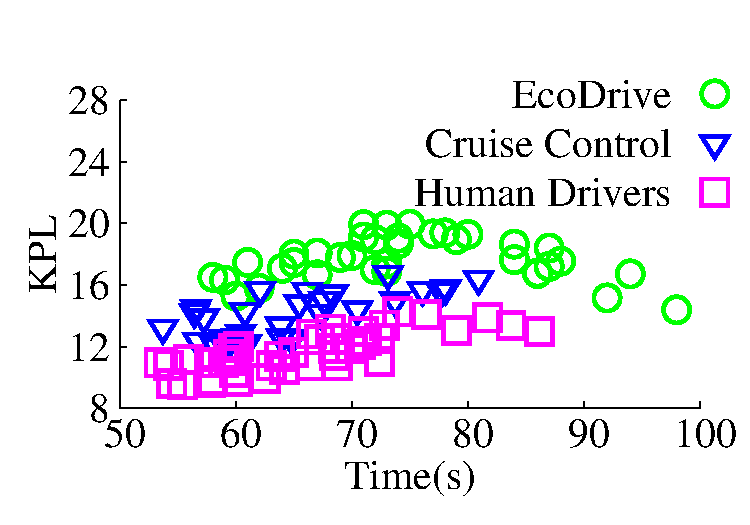
\includegraphics[width=3.0in,angle=0]{Figs/EcoDrive/evaluation/highway_timekpl.pdf}
\vspace{-0.0cm}
\caption{Tradeoff between travel time and fuel consumption on highway.}
\vspace{-0.6cm}
\label{tradeoff_highway}
\end{center}
\end{figure}

In this experiment, we evaluate the tradeoff between travel time and fuel consumption. 

\textbf{Urban}. 
The tradefoff between travel time and fuel consumption of EcoDrive on $250m$ 
road segment is shown in Fig. \ref{tradeoff_urban}. For EcoDrive, the optimal KPL is around 7 and the 
travel time is around 28 seconds. On the other hand, the average KPL for human 
drivers is around 5.5 and the average travel time is around 25 seconds. 
EcoDrive can achieve a 20\% fuel efficiency improvement 
on average by sacrificing travel time by around 10\%. 
EcoDrive can also improve fuel efficiency under same travel time in most cases. 

\textbf{Highway}.  
Fig. \ref{tradeoff_highway} shows the tradeoff between travel time and fuel efficiency on highway. 
Each highway segment length is around $2km-3km$. 
EcoDrive can improve fuel efficiency by more than 30\% on average without sacrificing travel time.    
The gain comes from smooth acceleration and road adaptation. 
More fuel efficiency can be achieved by cruising at the peak KPL speed, 
which is around $90km/h$ in this evaluation. 

\subsection{Modeling Accuracy}


\begin{figure}[!htbp]
\begin{center}
\vspace{-0.2cm}
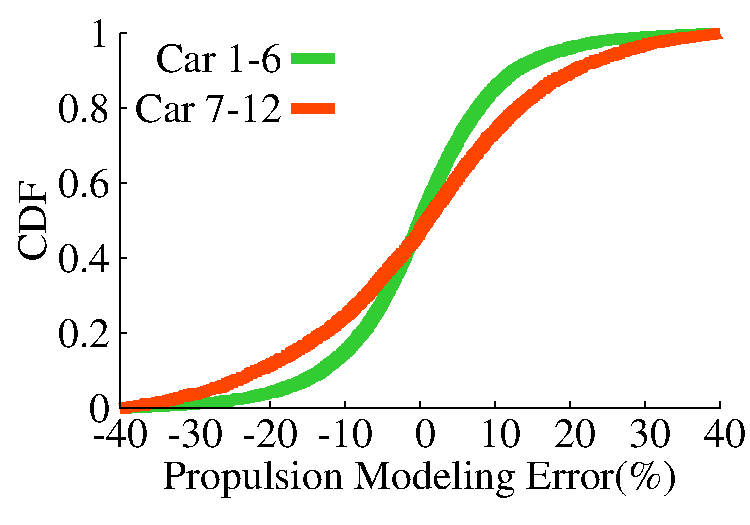
\includegraphics[width=2.2in,angle=0]{Figs/EcoDrive/evaluation/propulsion_error_cdf_2.pdf}
\vspace{-0.2cm}
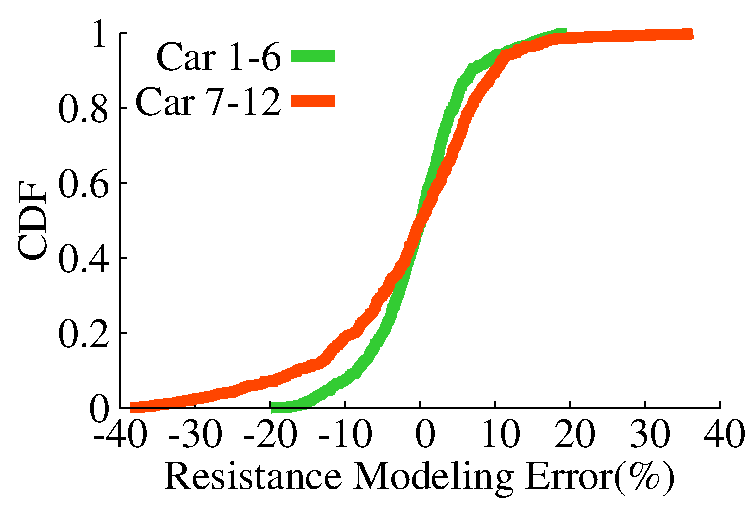
\includegraphics[width=2.2in,angle=0]{Figs/EcoDrive/evaluation/resistance_error_cdf_2.pdf}
\vspace{-0.2cm}
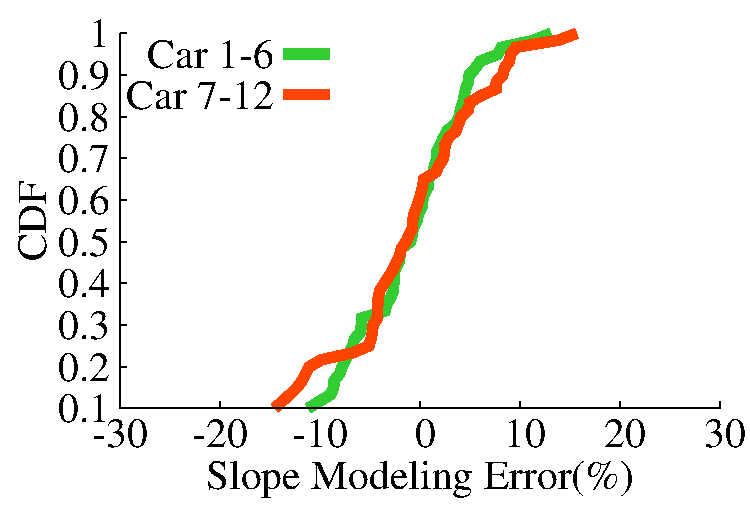
\includegraphics[width=2.2in,angle=0]{Figs/EcoDrive/evaluation/slope_error_cdf_2.pdf}
\vspace{-0.2cm}
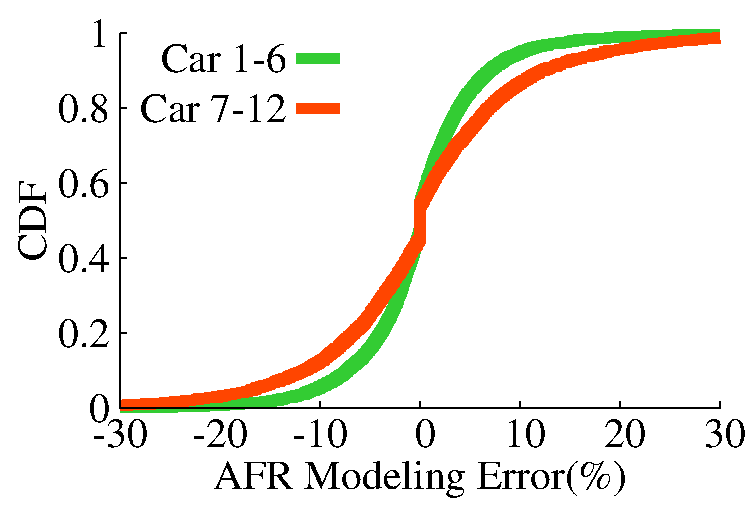
\includegraphics[width=2.2in,angle=0]{Figs/EcoDrive/evaluation/afr_profile_error_cdf_2.pdf}
\caption{The cumulative distribution function of vehicle dynamics modeling errors.}
\vspace{-0.6cm}
\label{modelingaccuracy}
\end{center}
\end{figure}

In this experiment, we evaluate the modeling accuracy of vehicle dynamics models. 
Different vehicle forces, propulsion, resistance and grade resistance, are
evaluated separately. 
The AFR profile calculation accuracy is evaluated as well. 
We divide the data into two sets, one set is the training set 
used to build the model and another set is the testing set
for evaluating the model. 
For each model, we repeat this process and plot the 
modeling accuracy of various vehicle dynamics models in Fig. \ref{modelingaccuracy}. 
From top-left to bottom-right, they are propulsion model evaluation, 
drivetrain loss and wind resistance model evaluation, 
grade resistance model evaluation, 
and AFR profile evaluation. 


We use \textcolor{green}{\textbf{green}} curves to represent the cars have more than one thousand miles
driving traces (Car 1-6) and use \textcolor{red}{\textbf{red}} curves to represent the rest (Car 7-12). 
The \textcolor{green}{\textbf{green}} curves show that the fitting errors of 
more than $95\%$ cases are within $\pm10\%$. 
The \textcolor{red}{\textbf{red}} curves show less fitting accuracy 
due to less miles. 




\subsection{Driving Data Statistics}

\subsubsection{Urban Road Segment Length}

\begin{figure}[!htbp]
\begin{center}
\vspace{-0.3cm}
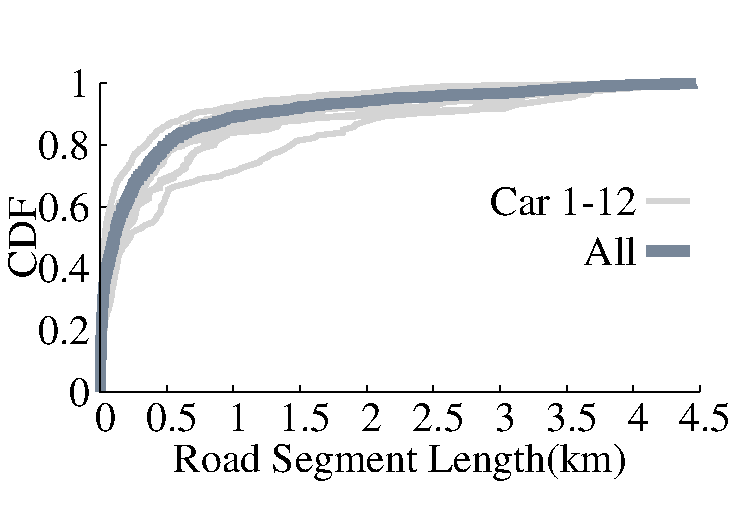
\includegraphics[width=3.0in,angle=0]{Figs/EcoDrive/evaluation/urban_road_segment.pdf}
\vspace{-0.0cm}
\caption{Road segment length in urban area.}
\vspace{-0.8cm}
\label{urbanroad}
\end{center}
\end{figure}

We summarize the length of road segments in Fig. \ref{urbanroad}.
A road segment is defined as the distance between two stand/stop locations. 
A stand/stop location is defined as following: 
1) The speed of the car is zero; 2) The car is making a turn. 
The speed of the car can be easily sensed from the OBD port. 
We identify turns from GPS data. 
The driving direction of car can be calculated from two adjacent GPS points. 
If the accumulated driving direction change are close to $90$ degree, 
then we mark this is a stand/stop location. 
This rough road segment length statistics give us a 
guideline for experiments. 
As shown in the figure, the most of road segments are within 1000m.
This indicates that the driving pattern in urban area is primarily  
accelerate-brake. 


\subsubsection{Urban Acceleration}



\begin{figure}[!htbp]
\begin{center}
%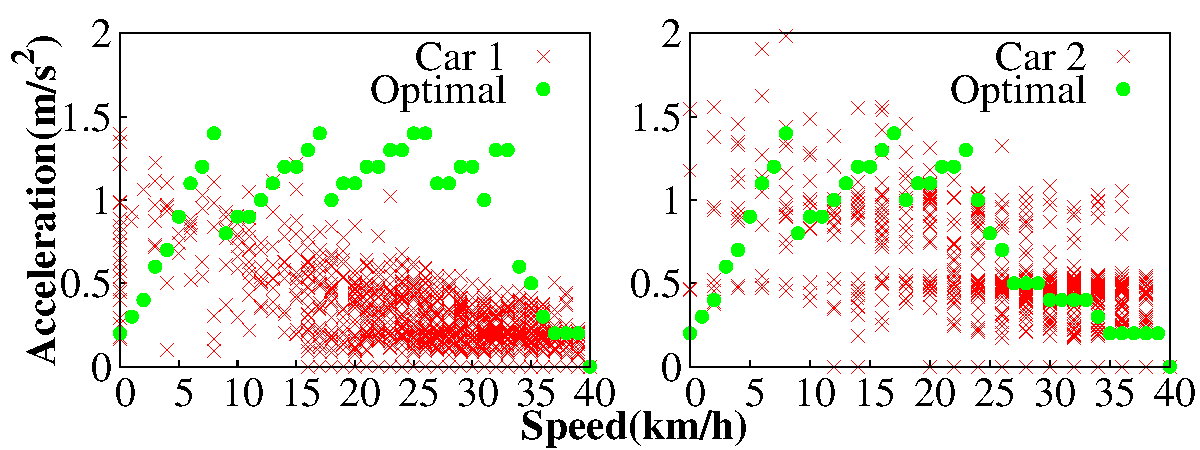
\includegraphics[width=3.2in,angle=0]{Figs/EcoDrive/evaluation/urban_accelerations.pdf}
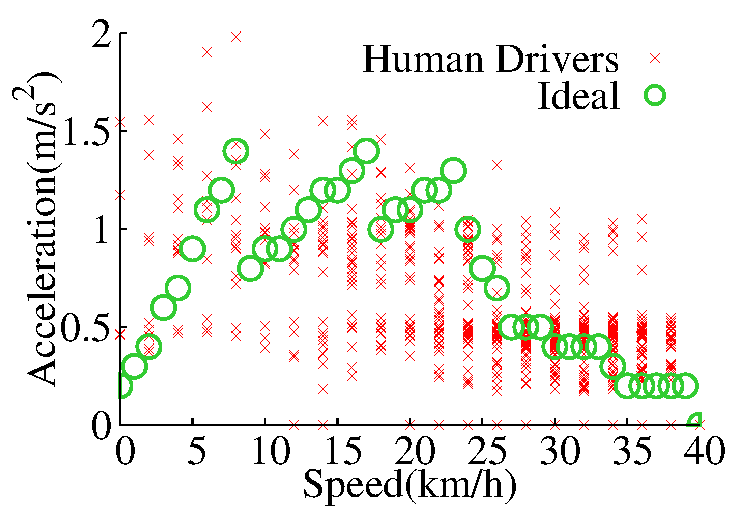
\includegraphics[width=3.0in,angle=0]{Figs/EcoDrive/evaluation/real_opt_acce_single.pdf}
\vspace{-0.0cm}
\caption{The urban acceleration patterns of different drivers.}
\vspace{-0.5cm}
\label{urbanaccelerations}
\end{center}
\end{figure}

Fig. \ref{urbanaccelerations} explains the acceleration patterns of
car 1 and the ideal acceleration pattern calculated by EcoDrive
with equal road length. 
As shown in the figure, drivers are not aware of the most efficient
accelerations of different speeds and not able to drive at a certain speed. 
They drive either lower than
desired accelerations, which will increase fuel consumption
due to longer travel time in low KPL speeds, 
or higher than desired accelerations, 
which will increase fuel consumption due to extra fuel consumption
to achieve the target speed. 



\subsubsection{Highway Driving Speed}






\begin{figure}[!htbp]
\begin{center}
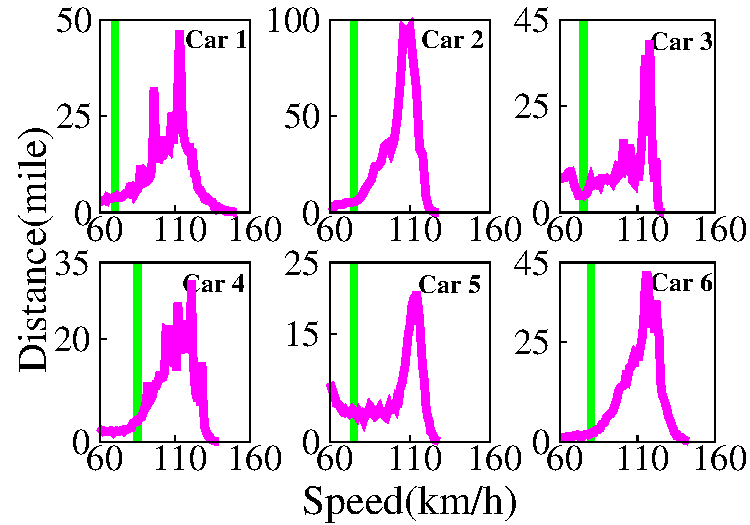
\includegraphics[width=3.0in,angle=0]{Figs/EcoDrive/evaluation/hwy_speeds.pdf}
\vspace{-0.0cm}
\caption{The highway driving speed distributions of car 1-6.}
\vspace{-0.6cm}
\label{highwayspeeds}
\end{center}
\end{figure}

The speed limits of rural highway is $65mph$ ($104.6km/h$) 
to $70mph$ ($112.6km/h$), and
the speed limit of urban highway is $55mph$ ($88.5km/h$). 
We summarize the highway driving speeds of car 1-6 
and illustrate the distribution and best KPL speed in Fig. \ref{highwayspeeds}. 
We observe that most drivers drive above the speed limits with
noticeable mileages and much higher than the best KPL speed. 
This is partially because the drivers are not aware of
the much higher fuel consumption in high speeds. 
Also, slowing down when following a slow car 
will increase fuel consumption due to power loss when braking. 
Frequent accelerations and decelerations increase
fuel consumption as well. 

\subsection{Trace-driven Simulation}


\begin{figure}[!htbp]
\begin{center}
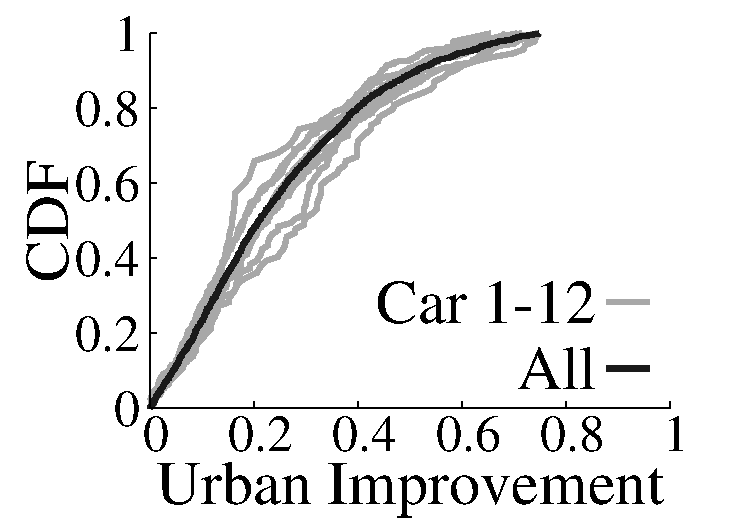
\includegraphics[width=2.0in,angle=0]{Figs/EcoDrive/evaluation/urban_cdf_all.pdf}
\hspace{-0.5cm}
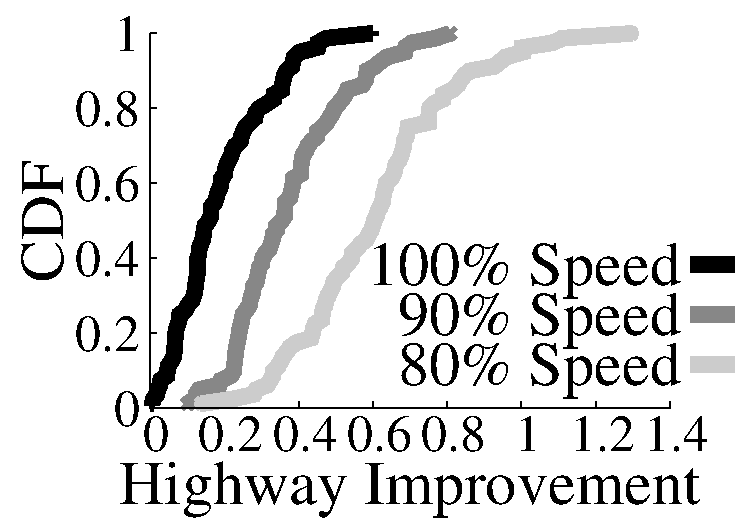
\includegraphics[width=2.0in,angle=0]{Figs/EcoDrive/evaluation/hwy_improve_cdf.pdf}
\vspace{-0.2cm}
\caption{Fuel efficiency improvements by trace-driven simulation.}
\vspace{-0.6cm}
\label{tracedriven}
\end{center}
\end{figure}

In this experiment, we evaluate EcoDrive by trace-driven simulations. 

\textbf{Urban}. We divide urban trips into variable-length road segments 
where the vehicular speed is 0 at the start and end of each segment. 
Each segment is divided into four parts, accelerating part, cruising part, 
braking part and idle part. 
Accelerating part ended when the speed does not increase in 5 seconds. 
Braking part started when the driver release gas pedal at the end of each segment. 
Cruising part falls between accelerating part and braking part.
Idle part follows braking part after the vehicular speed reach 0.  
The speed limit is calculated based on the average speed of cruising part. 
We calculate the fuel cost of EcoDrive by replaying acceleration and cruising parts.
We use the same braking and idle cost extracted from original traces.
We sum up the two costs to calculate the final fuel consumption of EcoDrive. 
As shown in Fig. \ref{tracedriven}, EcoDrive can improve a median of 
20\% fuel efficiency in urban environment. 
The travel time is reduced by 10\%-30\% in 20\% cases and is increased
by less than 25\% in 60\% cases. 
The plots of travel time are omitted due to the space limit.   

\textbf{Highway}.  
We divide highway trips into road segments based on deceleration.
If the deceleration is larger than a threshold, we separate current
segment into one highway segment.
The average speed of highway segment is used as target speed for EcoDrive. 
We replay each highway segment by EcoDrive with three different
target speeds, the same target speed, 90\% of target speed and
80\% of target speed. 
As shown in Fig. \ref{tracedriven}, EcoDrive can improve
fuel efficiency by more than 20\% on average without sacrificing 
travel time and can improve an average of 40\% fuel efficiency
by sacrificing 10\% travel time on highway. 


   

 


\section{Issues and Discussion}


In this section, we discuss some design considerations of EcoDrive. 


\textbf{Hybrid Vehicle (HV) and Electric Vehicle (EV)}. 
EcoDrive is designed for gasoline-powered vehicles, but the modeling process
and gas pedal emulation can also be applied to HVs and EVs. 
Currently, the majority of vehicles running
on street are still gasoline-powered vehicles. 
It is important to develop systems like EcoDrive
to work on regular vehicles to improve fuel efficiency
and limit carbon pollution. 
The core of EcoDrive is that it can work on regular vehicles
with easy and recoverable installation. 


\textbf{Instant Fuel Economy Display}.
In urban environments, acceleration is not fuel efficient, but accelerating to a higher speed
in a careful way can improve fuel efficiency. 
If the driver refuses to accelerate due to low instant fuel efficiency,
the car will drive in low fuel efficient speed and eventually increase
fuel consumption. 
Similarly, releasing gas pedal can increase instant fuel efficiency dramatically, 
but frequent acceleration and deceleration will consume more fuel
than cruising under certain speed. 
Therefore, instant fuel economy display is misleading
and may reduce overall fuel efficiency. 



\textbf{Impact of Traffic and User Experience}.
EcoDrive controls the vehicle in a way that is similar to cruise control, 
so the driver should keep a safe distance to
front vehicle. 
Since EcoDrive accelerates the vehicle in various ways according to
different road segment lengths, 
it is more challenging for human drivers to keep safe distance than cruise
control in dense traffic scenarios, because
drivers need to frequently brake to avoid front-end collision. 
Therefore, EcoDrive is more suitable for drivers to use in low traffic volume scenarios. 
However, it is shown from the data we collected that drivers tend to
accelerate much more aggressive than the optimal acceleration patterns. 
In other words, EcoDrive achieves higher fuel efficiency by accelerating
slower than most drivers usually do. 
Also, EcoDrive uses fixed acceleration pattern for fixed road length
and speed limit, 
drivers and passengers can easily get used to the driving style
of EcoDrive. 
Therefore, we expect EcoDrive can be useful in most urban driving scenarios 
(except traffic hours) and drivers can still feel that the vehicles are under control
due to predictable accelerations. 
We also expect that EcoDrive can tolerate more complex traffic
conditions when integrating with front object detection and
route planning systems equipped on driverless cars. 


\textbf{Limitations}. 
First, EcoDrive requires the road length as input in short length road segment 
(e.g., shorter than 200m). 
Second, it relies on drivers to brake or switch to disable EcoDrive mode. 
The operation complexity is acceptable for drivers as proven
by cruise control.
Third, EcoDrive requires mileage trainings to build an accurate model, i.e., 
1000 miles driving data can build a very accurate model as shown in evaluation. 
Some optimization can be made to reduce training time, e.g., sharing the AFR profile 
among same vehicle models.
Fourth, we did not evaluate EcoDrive by end-to-end scenarios in urban environment, 
e.g., what are the fuel savings from home to work. 
There are different traffic volumes 
and different traffic light schedules among different trips. 
Therefore, it is challenging to compare EcoDrive with human drivers 
in such scenarios. 
Given the fuel improvement in arbitrary length road segments, 
we believe EcoDrive can improve fuel efficiency in end-to-end scenarios as well.   

Each trip can be divided into three parts: acceleration, cruising and braking. 
Acceleration and cruising consume most of the fuel during a trip. 
For this work, EcoDrive focuses on the acceleration part and cruising part. 
There is no direct way to fairly compare two brakes that made by different drivers, 
or different brakes made by the same driver. 
Therefore, we did not include the fuel consumption of braking in our evaluation. 

There are other factors that affect fuel consumption, e.g., 
tire pressure, temperature and wind direction etc. 
A more accurate model can be built by using more 
vehicle parameters. 
However, there is no direct way to access some in-vehicle parameters
like tire pressure. 
We advocate that the vehicle manufacturers provide more
information through OBD port that can be used to enable
more applications. 
Some other real world parameters, 
e.g., traffic light schedule, stop sign and wind direction etc., 
can also be used to improve fuel efficiency. 
We believe such extra information can be used to improve 
EcoDrive in broader aspects.





\section{Summary of EcoDrive}

This paper introduces EcoDrive, a fuel consumption sensing and control
system that assists human driver to drive fuel efficiently. 
EcoDrive calculates driving strategy based on the properties of individual vehicles 
and road conditions. 
To this end, it models vehicle dynamics as functions of instant fuel consumption
and calculates acceleration strategies accordingly. 
We build a prototype of EcoDrive on a mobile embedded platform. 
The prototype is installed on a regular vehicle and
tested for more than 100 miles in both urban and highway environments. 
In comparison with human drivers, 
EcoDrive improves fuel efficiency by 10\%-40\% in urban environments. 
It has an average of 10\% higher fuel efficiency than vehicle built-in cruise control
and more than 30\% fuel efficiency than human drivers
on highway.  





